\documentclass[a4paper, 12pt]{article}
\usepackage[T1]{fontenc}
\usepackage[utf8]{inputenc}
\usepackage[english]{babel}
\usepackage{graphicx}
\usepackage[style=ieee, backend=biber]{biblatex}
%\usepackage[hidelinks]{hyperref}
\usepackage{hyperref}
\usepackage{float}
\addbibresource{bib.bib}
\usepackage{setspace}
\usepackage{amsfonts}
\usepackage[nottoc,numbib]{tocbibind}
\usepackage{amsmath}
\numberwithin{equation}{section}


\DeclareMathOperator*{\argmax}{arg\,max}

\onehalfspacing

\begin{document}

\title{Flatland Challenge}
\author{G. Berselli, R. De Matteo, M. M. L. Pulici}
\date{July 19, 2021}
\maketitle
\begin{center}
	\fbox{
\includegraphics[width=\textwidth]{Images/Flatland_Logo.jpg}}
\end{center}


\clearpage

\tableofcontents

\clearpage

\listoffigures

\clearpage


\section[Flatland Challenge]{Flatland Challenge \cite{flatland}}

The aim of the challenge, is to achieve efficient management of railway traffic. In particular, this problem is tackled in a simple grid world environment, in order to simulate and experiment different scenarios.

In more detail, the goal consists in making a number of trains arrive at their destinations minimizing the travel time. Even though for simple environments the train can follow explicit plans, as complexity increases the problem of mapping all possible states becomes intractable, for this reason a class of algorithms known as Reinforcement Learning (Section \ref{sec:reinforcement-learning}) can be exploited.

\begin{figure}[h]
	\centering
		\fbox{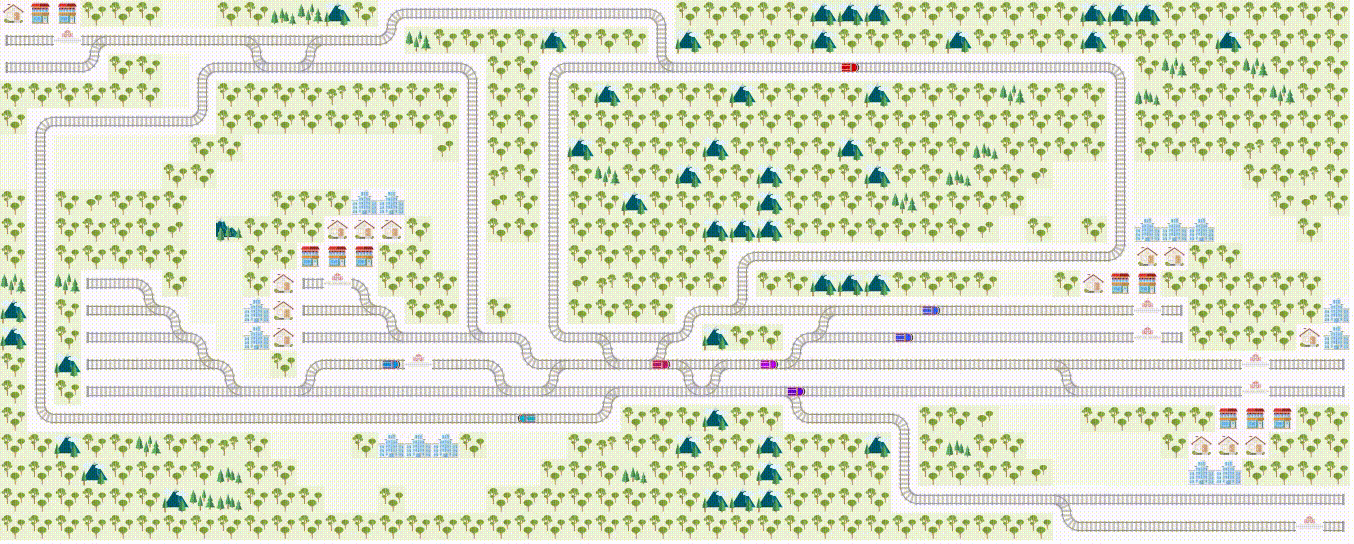
\includegraphics[width=\textwidth]{Images/Flatland_Example.png}}
		\caption{A possible Flatland instance}
\end{figure}

\subsection[The environment]{The environment \cite{flatland-challenge}}

The Flatland environment consists in a discrete time simulation, meaning that each action is performed with a constant time step. At each step, an agent for each simulated train chooses an action. An agent is defined as an entity that can move within the grid and must solve tasks. More precisely, each agent can choose between two actions: waiting or moving in a direction. Each agent has an individual starting position and its goal is to reach its target destination. Of course, two agents can not occupy the same cell at the same time.

Each cell in the Flatland grid can take the form of any of 8 tile types, as shown in Fig. \ref{fig:cell-types}. More configurations can be obtained by rotating and mirroring the 8 basic tiles.

\begin{figure}[h]
	\centering
		\fbox{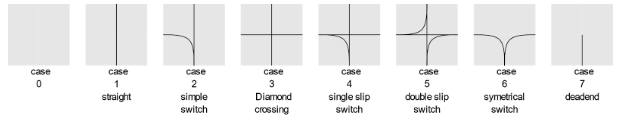
\includegraphics[width=\textwidth]{Images/cell-types.png}}
		\caption{The 8 cell types}
	\label{fig:cell-types}
\end{figure}

When the tile is of the straight type, the agent can only choose to continue moving or to stop. In presence of a simple or a double switch, the train is forced to decide in which of the offered direction to move. When arriving at a dead end, an agent can only stop or go backward.


\subsection[Actions]{Actions \cite{actions-rewards}}

Since Flatland is a railway simulations, the agents' actions are naturally very limited. In particular, there are 5 basic actions:
\begin{itemize}
	\item \texttt{DO\_NOTHING}: if moving, the agent keeps moving, if stopped, it stays stopped;
	\item \texttt{MOVE\_LEFT}: if the agent is at a switch with a leftward transition, it chooses the left path, otherwise it does nothing;
	\item \texttt{MOVE\_FORWARD}: if the agent is at a switch with a straight transition, it goes straight, otherwise it does nothing;
	\item \texttt{MOVE\_RIGHT}: if the agent is at a switch with a rightward transition, it chooses the right path, otherwise it does nothing;
	\item \texttt{STOP\_MOVING}: the agent stops.
\end{itemize}


\subsection[Observations]{Observations \cite{observations}}

The Flatland environment comes with 3 default observation: Global, Local Grid, and Local Tree. A graphical representation of the 3 observations is given in Fig. \ref{fig:observations}.

\begin{figure}[h]
	\centering
		\fbox{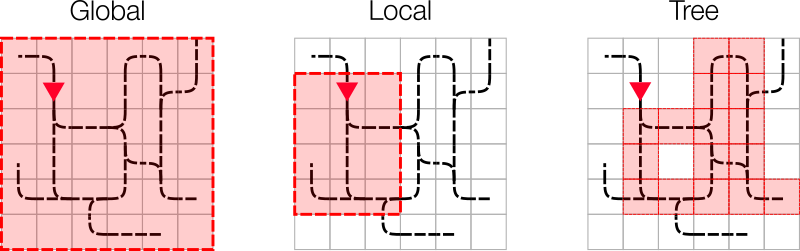
\includegraphics[width=\textwidth]{Images/observations.png}}
		\caption{The 3 default Flatland observations}
	\label{fig:observations}
\end{figure}


\subsubsection{Global Observation}

The Global Observations returns the entire rail environment. In more details, it is composed of:
\begin{itemize}
	\item Transition map: provides a unique value for each type of transition map and its orientation;
	\item Agent state: a 3D array containing:
	\begin{itemize}
		\item Channel 0: a one-hot encoding of the self agent's position and direction;
		\item Channel 1: other agents' positions and directions;
		\item Channel 2: self and other agents' malfunctions;
		\item Channel 3: self and other agents' speeds;
		\item Channel 4: the number of other agents ready to depart from that position;
	\end{itemize}
	\item Agent targets: a 3D array containing the position of the self agent target and the positions of the other agents' ones.
\end{itemize}

\subsubsection{Local Grid Observation}

The Local Grid Observation returns the rail environment in a neighborhood of the agent. Its features are similar to that of the Global Observation, but the view field of the agent is limited. The main advantage over the Global Observation is that the Local Grid Observation reduces the amount of irrelevant information. In addition, it features a distance map, which gives information about the distance of each agent from its target.


\subsubsection{Tree Observation}

The Tree Observation exploits the graph structure of the railway. It generates a 4-branched tree starting from the agent's position, with each branch following an allowed transition. More information can be found in Section \ref{sec:tree-observation}.


\subsection[Rewards]{Rewards \cite{actions-rewards}}

At each time step, each agent receives combined local and global rewards. At a local level, a reward $r_l=-1$ is given to each agent until its target location is reached. After this happens, the agent will receive a constant reward of $r_l=0$. The global reward, on the other hand, by default starts at $r_g=0$ and turns to $r_g=1$ only after all agents have reached their targets. In total, the agent $i$ receives a reward:
\begin{equation}
	r_i\left(t\right)=r_l\left(t\right)+r_g\left(t\right).
\end{equation}




\subsection[Malfunctions]{Malfunctions \cite{malfunctions}}

Malfunctions are introduced in the Flatland environment in order to simulate stochastic events. In real life, the initial scheduling plan often needs to be changed because of unexpected events such as delayed arrivals or various other malfunctions. The way malfunctions are implemented is by using a Poisson process to stop agents at random times for random durations.

\subsection[Speed profiles]{Speed profiles \cite{speeds}}

In a real railway, the difference in the various agents' speeds plays a huge role in increasing the complexity of the system. In Flatlands, this is simulated by using different speed profiles: a fastest speed is set to be $1$, and all trains can take fractional speed values between $0$ and $1$.











\clearpage
\section[Reinforcement Learning]{Reinforcement Learning \cite{reinforcement-learning}}\label{sec:reinforcement-learning}

The term Reinforcement Learning refers to the class of agents which rely on feedbacks, or rewards, produced by the agents themselves when interacting with the environment. The way Reinforcement Learning works is to use observed rewards to learn the best possible policy for the given environment. In other words, the agent has no prior knowledge of the environment and must learn how to behave based only on posterior trial-and-error feedbacks.

There are three basic agent designs for Reinforcement Learning:
\begin{itemize}
	\item Utility-based agent, which learns a utility function on states and uses it to select actions;
	\item Q-learning, which learns an action-utility function giving the expected utility of an action given a state;
	\item Reflex agent, which learns a policy mapping directly from states to actions.
\end{itemize}

In addition to these designs, Reinforcement Learning can be either passive, meaning that the policy is fixed and the task is to learn the utilities of states, or active, referring to agents which must also learn how to act.

\subsection[Q-learning]{Q-learning \cite{dqn-tutorial}}

For the Flatland Challenge, Q-learning is used. This class of algorithms learns an action-utility representation instead of simply learning the utilities. The value of an action-state tuple is typically indicated as $Q\left(s,a\right)$. There is a direct correlation between Q-values and state utilities, as expressed by the following equation:
\begin{equation}
	U\left(s\right) = \max_a Q\left(s,a\right).
\end{equation}

The main difference between Q-functions and basic utility information si that no model of the form $P\left(s'|s,a\right)$ is needed, either for learning or for action selection. This characteristic makes Q-learning a model-free method.

The basic Q-learning algorithm is composed of the following steps:
\begin{enumerate}
	\item Q-table initialization;
	\item Action selection;
	\item Q-table update.
\end{enumerate}


A Q-table is a data structure which is used to keep track of the visited state-action pairs and the corresponding expected Q-values. At the very beginning of the learning process, the Q-table is filled with zeros, which represent the agent's lack of knowledge about the environment.

From here, the agent employs a trial-and-error strategy, choosing actions and balancing between exploration of new states and exploitation of previously collected knowledge. The way these actions are chosen depend on the so-called action selector, whose different types are explored in Section \ref{sec:action-selectors}.


The third steps consists in updating the Q-table using the Bellman Equation:
\begin{equation}\label{eq:bellman}
	Q\left(s,a\right)\leftarrow \left(1-\alpha\right)Q\left(s,a\right)+\alpha\left(r+\lambda\max_{a'}Q\left(s',a'\right)\right),
\end{equation}
where $s$ is the current state, $a$ is the action taken, $r$ is the reward for the taken action, $\alpha$ is the learning rate parameter and $\lambda$ is the discount factor. The last $\max$ operation is performed on all actions $a'$ which can be taken from the updated state $s'$.


A close alternative to standard Q-learning can be found in the \textsc{Sarsa} (State-Action-Reward-State-Action) algorithm. The concept is very close to that of Q-learning, but Eq. \eqref{eq:bellman} is replaced by:
\begin{equation}\label{eq:sarsa}
	Q\left(s,a\right)\leftarrow \left(1-\alpha\right)Q\left(s,a\right)+\alpha\left(r+\lambda Q\left(s',a'\right)\right).
\end{equation}

The only difference between Eqs. \eqref{eq:bellman} and \eqref{eq:sarsa} is that $\max_{a'}Q\left(s',a'\right)$ is simply replaced by $Q\left(s',a'\right)$. In other words, instead of the maximum of the possible Q-values from the state reached in the transition, the actual value of the state $s'$ reached after taking action $a'$ is used. The value update takes place once at the end of each $s$, $a$, $r$, $s'$, $a'$ cycle, as suggested by the name.

If the agent is a greedy one, always choosing the action with the best Q-value, there is no difference between the two algorithms. If, on the other hand, there is some exploration happening, there is a crucial difference: Q-learning is said to be an off-policy algorithm, because it does not care about the policy used; \textsc{Sarsa}, on the contrary, is considered on-policy. Even though Q-learning is more flexible, being able to learn well even with bad exploration policies, it is not as realistic, since it does not take into consideration possible external uncontrollable events.


\subsection[Multi-Agent Reinforcement Learning]{Multi-Agent Reinforcement Learning \cite{multi-agent-rl}}

Multi-Agent Reinforcement Learning (\textsc{Marl}) refers to a version of Reinforcement Learning where multiple agents interact in a common environment. There are three main broad categories which classify \textsc{Marl}:
\begin{itemize}
	\item Cooperative: when all agents have a common goal and work together;
	\item Competitive: when agents compete to accomplish a goal;
	\item Mixed: when agents are grouped in teams, with intra-group cooperation and inter-group competition.
\end{itemize}


\clearpage
\section{Implementation}



\subsection[Deep Q-Network Agents]{Deep Q-Network Agents \cite{dqn-tutorial, improvements, drl-8-dqn-ddqn}}\label{sec:dqns}

Learning using Deep Q-Networks (DQN) is a relatively new paradigm, having been introduced in 2014. In general, the main feature of DQN algorithms is the exploitation of Deep Neural Networks to learn the Q-values of a problem. There are many versions of DQN algorithms, of which the most common are:
\begin{itemize}
	\item Standard DQN;
	\item Double DQN;
	\item Dueling DQN.
\end{itemize}


\subsubsection{Standard DQN}

The basic DQN algorithm closely resembles the standard Q-learning one, consisting of:
\begin{enumerate}
	\item Neural network(s) initialization;
	\item Action selection;
	\item Network weights update.
\end{enumerate}

The main difference between DQN and standard Q-learning is the way the Q-table is implemented. Rather than mapping the state-action pair to a Q-value, the neural network maps input states to action-value pairs.

Again, Eq. \eqref{eq:bellman} is used to update the neural networks. In particular, the change of weights is expressed by:
\begin{equation}\label{eq:weights}
	\Delta w = \alpha\left[\left(r+\lambda\max_{a'} Q\left(s',a',w\right)\right)-Q\left(s,a,w\right)\right]\nabla_wQ\left(s,a,w\right),
\end{equation}
where the part in the square brackets represent the temporal difference error and the last factor is the gradient of the current predicted Q-value.





\subsubsection{Double DQN}

When Eq. \eqref{eq:bellman} is used in a Neural Network, the same parameters are used for estimating both the target and the Q-value. This is an issue, since it means that there is a big correlation between the target and the changing parameters: at every step, both the Q-values and the target values shift, leading to big oscillations in training.

A possible solution is to use the so-called Double DQN. The aim of this approach is to tackle the problem of checking that the best action for the next state is the one with the highest Q-value. In general, the accuracy of Q-values depend on both the action chosen and what states have been explored. Therefore, at the beginning of the training there is no information about the best action to take: taking the maximum Q-value can lead to false positives. This natural tendency of DQN to given higher Q-values to suboptimal actions complicates learning.

The Double DQN approach tries to fix this problem by using two separate networks to decouple the action selection from the target Q-value generation. First, the DQN network is used to select the best action to take for the next state, then the target network calculates the target Q-value of the state-action combination. So, the Double DQN method reduces Q-value overestimation and makes training faster and stabler. Practically, the time difference target $Q\left(s,a\right)$ becomes:
\begin{equation}
	Q\left(s,a\right)=r+\lambda Q\left(s',\argmax_{a'}Q\left(s',a'\right)\right).
\end{equation}

Then, every $\mathrm{T}$ steps the weights $w^-$ of the target network are updated with the DQN network ones $w$:
\begin{equation}
	w^-\leftarrow w.
\end{equation}

An alternative to this weight updating method is given by the so-called soft update \cite{soft-update}. The term soft update refers to an approach which does not update the weights once every $\mathrm{T}$ steps, but rather frequently and very little every time. In particular, new weights are given by:
\begin{equation}
	w^-\leftarrow w\tau+w^-\left(1-\tau\right),
\end{equation}
where $\tau$ is an arbitrary (small) parameter.


\subsubsection{Dueling DQN}

The third DQN version is based on decomposing the Q-value in two parts, as shown in Fig. \ref{fig:dueling}:
\begin{equation}
	Q\left(s,a\right)=V\left(s\right)+A\left(s,a\right)
\end{equation}
where $V\left(s\right)$ is the value of being in state $s$ and $A\left(s,a\right)$ is the advantage of taking action $a$ at state $s$. To be more precise, the actual equation used is:
\begin{equation}
	Q\left(s,a\right)=V\left(s\right)+A\left(s,a\right)-\frac{1}{\left|A\right|}\sum_aA\left(s,a\right),
\end{equation}
where the last term is a normalization factor.

\begin{figure}[h]
	\centering
		\fbox{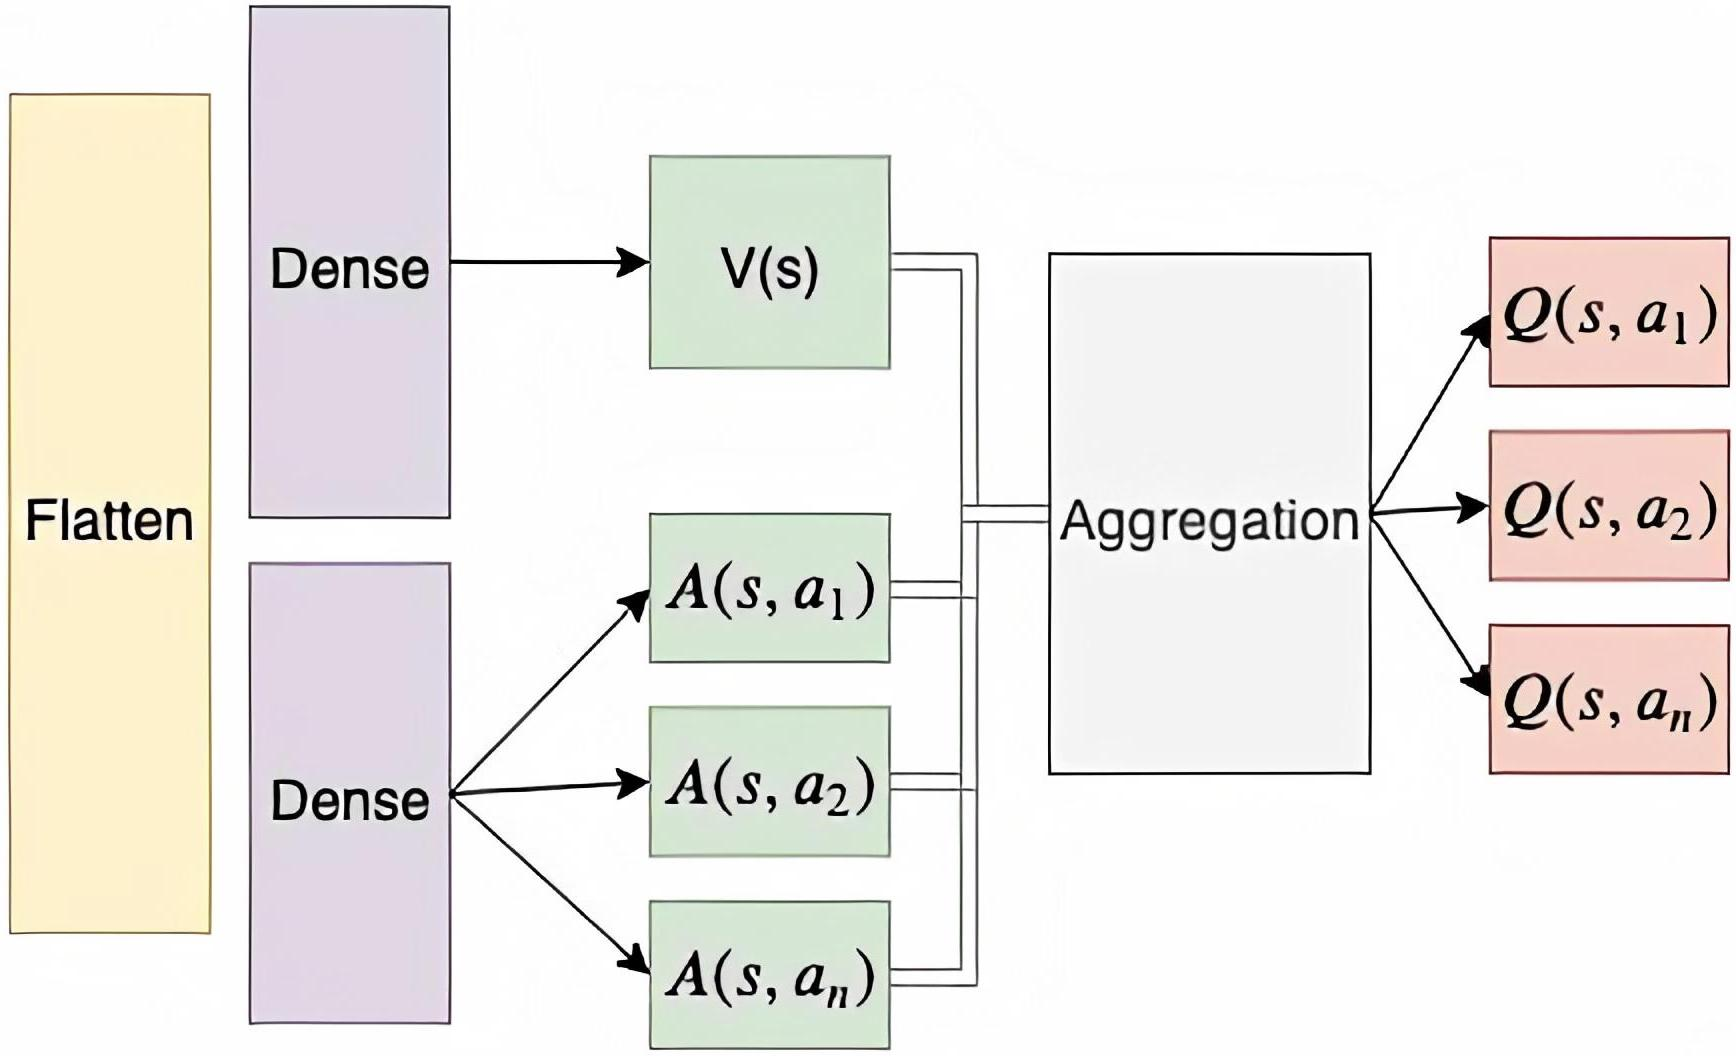
\includegraphics[width=\textwidth]{Images/dueling.jpg}}
		\caption{A schematic of the Dueling DQN}
	\label{fig:dueling}
\end{figure}

Dueling DQN focuses on separating the estimator of the two values, using one stream to estimate the state value $V\left(s\right)$ and another one to estimate the advantage of each action $A\left(s,a\right)$. Decoupling these two values becomes particularly useful for states where any action does not affect the environment in a relevant way.




\subsubsection{Further DQN approaches}

Of course, these three methods are not the only ones to deal with DQNs. A particularly exhaustive analysis of all the different improvements to the DQN algorithm is represented by the seminal work by Hessel et al. \cite{rainbow}: in the paper, different DQN approaches are compared, culminating in the creation of a state-of-the-art integrated ``Rainbow'' agent, exploiting all the advantages of the most successful approaches.% These results are shown as a reference in Fig. \ref{fig:rainbow}.


%\begin{figure}[h]
%	\centering
%		\fbox{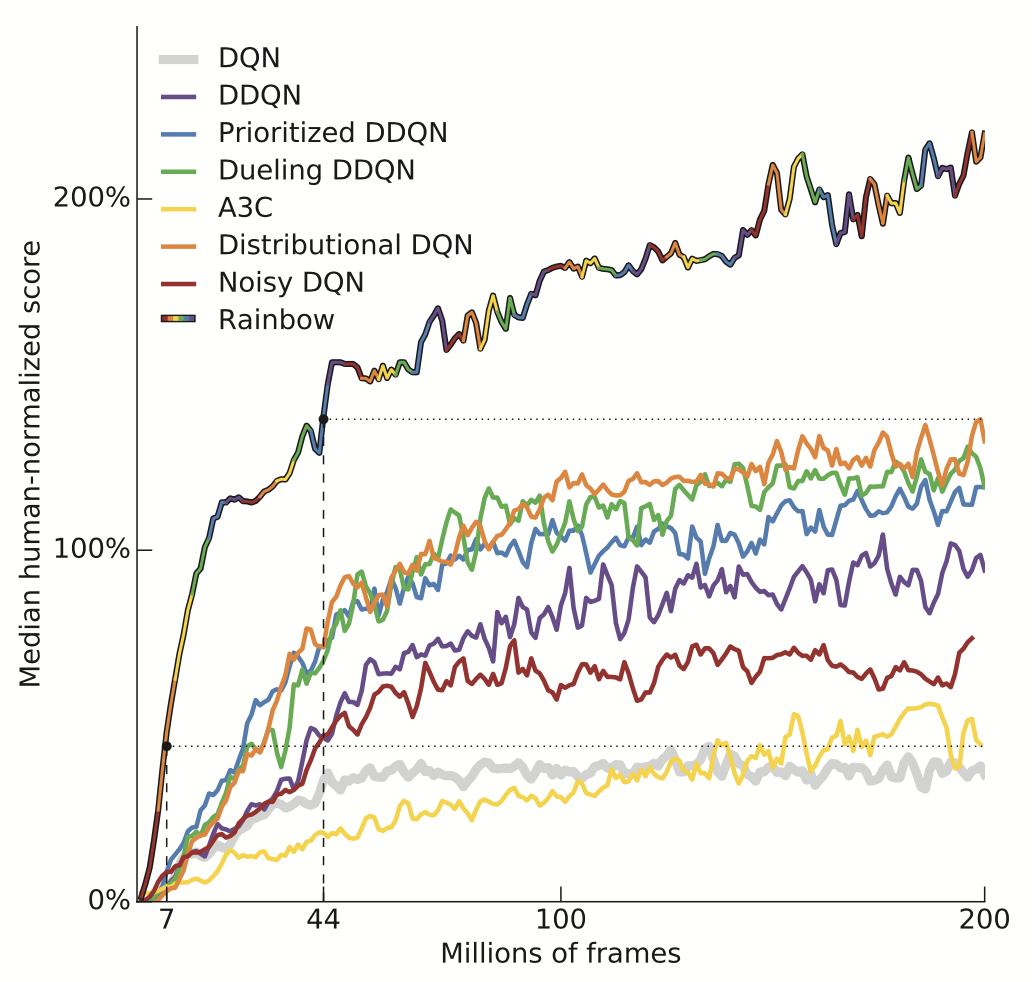
\includegraphics[width=\textwidth]{Images/rainbow.png}}
%		\caption{Comparison of various DQN approaches, including the state-of-the-art Rainbow agent.}
%	\label{fig:rainbow}
%\end{figure}













\subsection[Action Selectors]{Action Selectors \cite{action-selectors}}\label{sec:action-selectors}
In the learning process of a Reinforcement learning agent, exploration plays a crucial role: in order for an agent to properly learn from the interaction with the environment, it must be exposed to as many states as possible. Since an agent needs the right experiences to learn a good policy, but also needs a good policy to obtain the environment, a balance, known as exploration-exploitation tradeoff, needs to be reached. There are various action selection approaches which can be used by the agent, of which the main ones are:
\begin{itemize}
	\item Random Approach;
	\item Greedy Approach;
	\item $\varepsilon$-Greedy Approach;
	\item Boltzmann Approach;
	\item Noisy Approach.
\end{itemize}


\subsubsection{Random Approach}

The Random Approach is the most basic method of selecting an action: the agent does not use any prior knowledge and picks randomly among all the possible actions. This approach is illustrated in Fig. \ref{fig:random}.

\begin{figure}[h]
	\centering
		\fbox{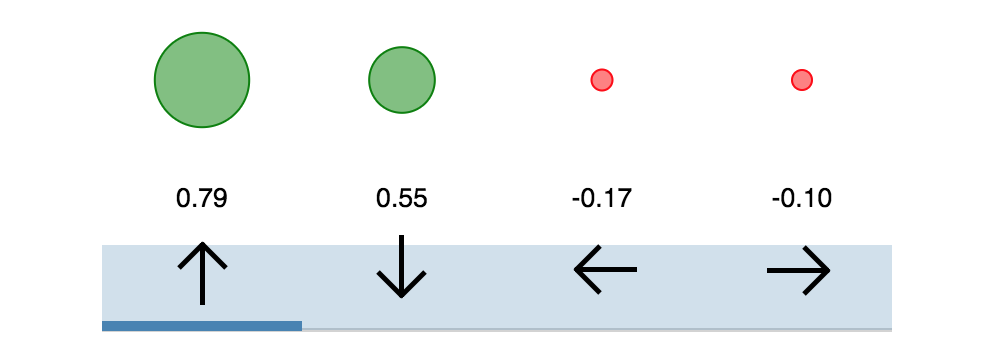
\includegraphics[width=\textwidth]{Images/random.png}}
		\caption{Action selection distribution for the Random Approach}
	\label{fig:random}
\end{figure}

Despite providing a lot of exploration, this approach is obviously deficient in exploiting the knowledge already learned by the agent.


\subsubsection{Greedy Approach}

The Greedy Approach is the extreme opposite of the Random one: it consists in always opting for the action with the highest Q-value, regardless of the values of the other choices. This approach is illustrated in Fig. \ref{fig:greedy}.

\begin{figure}[h]
	\centering
		\fbox{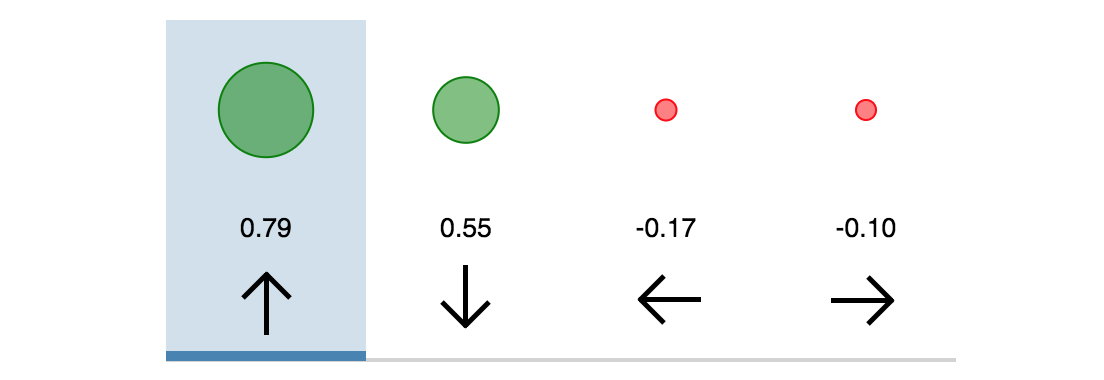
\includegraphics[width=\textwidth]{Images/greedy.png}}
		\caption{Action selection distribution for the Greedy Approach}
	\label{fig:greedy}
\end{figure}

At first, this approach might appear good, as the agent always opts for the action it thinks to be the best. The main shortcoming of this method is that it almost always provides a suboptimal solution, since no alternate solutions are explored. In other words, in Greedy Approach, exploitation is favored enormously over exploration, which is almost absent. 





\subsubsection{$\varepsilon$-Greedy Approach}

The $\varepsilon$-Greedy Approach can be viewed as a combination of the Greedy and the Random ones. The way the agent acts in this case is by always opting for the optimal action, except occasionally it acts randomly. The choice between the two approaches is dictated by an adjustable parameter $\varepsilon$, which represents the probability to act randomly. This approach is illustrated in Fig. \ref{fig:epsilon}.

\begin{figure}[h]
	\centering
		\fbox{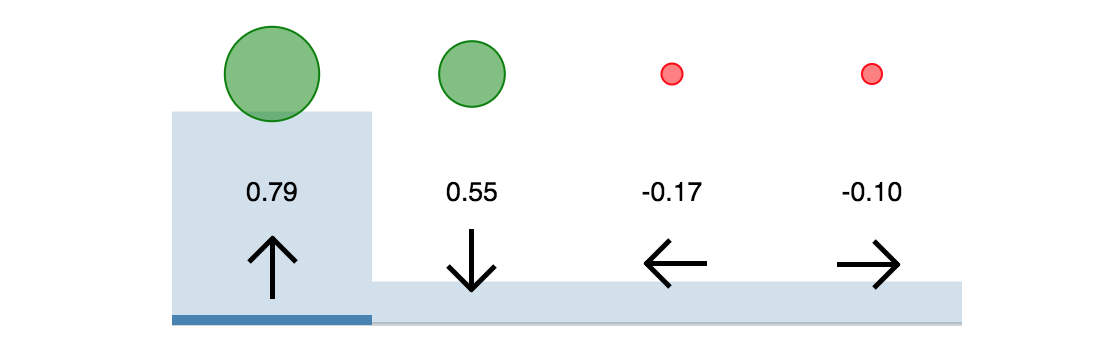
\includegraphics[width=\textwidth]{Images/epsilon.png}}
		\caption{Action selection distribution for the $\varepsilon$-Greedy Approach}
	\label{fig:epsilon}
\end{figure}

This approach encountered a huge success due to its combination of simplicity and power: even though it is only a mixture of two very mediocre methods, the performance improvement is remarkable. To further enhance the agent's learning ability, the value of $\varepsilon$ is often adjusted during training: in the beginning it starts as a big value, in order to provide maximum exploration, and it is slowly annealed as the agent obtains more information about the environment. The only shortcoming of the $\varepsilon$-Greedy Approach is that it only takes into account whether an action is the most rewarding or not, making it not optimal.


\subsubsection{Boltzmann Approach}

The Boltzmann Approach takes the exploration-exploitation balance of $\varepsilon$-Greedy even further: instead of always taking the optimal action or acting randomly, it chooses among the various actions using individual Q-values to weigh probabilities. This approach is illustrated in Fig. \ref{fig:boltzmann}.


\begin{figure}[h]
	\centering
		\fbox{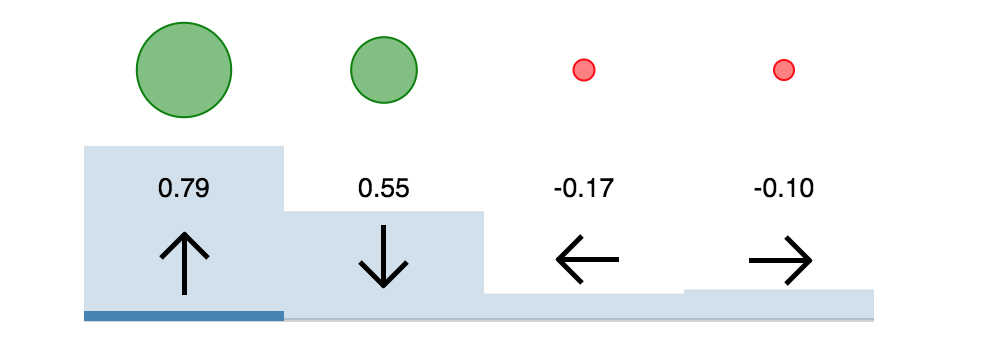
\includegraphics[width=\textwidth]{Images/boltzmann.png}}
		\caption{Action selection distribution for the Boltzmann Approach}
	\label{fig:boltzmann}
\end{figure}

Compared to $\varepsilon$-Greedy, the Boltzmann Approach also takes into consideration the information about the values of actions other than the optimal: this way, actions which are potentially promising are given a higher priority over clearly inferior choices.

An interesting feature of the Boltzmann Approach is the use of an additional temperature parameter $\tau$, which is annealed over time in a fashion similar to the way $\varepsilon$ is treated. The $\tau$ parameter controls the probability distribution of the actions using the thermodynamics Boltzmann equation, which gives the name to the approach:
\begin{equation}\label{eq:boltzmann}
	P\left(a\right) = \frac{\mathrm{e}^\frac{Q\left(a\right)}{\tau}}{\sum_{i=1}^n \mathrm{e}^\frac{Q\left(a_i\right)}{\tau}},
\end{equation}
where $P\left(a\right)$ is the probability of choosing action $a$, and $a_i$ are all the possible action choices.

The main problem of this approach is that it builds on the assumption that the probability distribution outlined in Eq. \eqref{eq:boltzmann} provides a measure of the agent's confidence in action $a$, while in reality what the agent is estimating is a measure of how optimal the agent thinks the action is, not how certain it is about that optimality.



\subsubsection[Noisy Approach]{Noisy Approach \cite{deep-reinforcement, noisy}}

The Noisy Approach is somewhat different from all the others: instead of acting on the probability of the agent choices, it adds some noise to the output of the Neural Network itself. In particular, the basic Noisy Approach consists in adding some gaussian node to the last layers of the network using the formula:
\begin{equation}
	w_i = \mu+\sigma\cdot\varepsilon
\end{equation}
where $\mu$ is a variable with random initialization, $\sigma$ is a variable with constant initialization, and $\varepsilon$ is the noise with a random value between $0$ and $1$.

There are two main ways of introducing noise to the Network: Independent Gaussian Noise and Factorized Gaussian Noise. Using the first method, every weight of the noisy layer is independent, with its own $\mu$ and $\sigma$. The Factorized version, on the other hand, uses two vectors: the first one has the same length as the input, the second one the same as the output. A special function is then applied to both vectors and a matrix multiplication between them is calculated and is then used to add weights.



\subsection[Experience Replay]{Experience Replay \cite{experience-replay}}\label{sec:experience-replay}

In basic Q-learning algorithms, experiences are utilized just once and then thrown away. This is a waste, as some experiences may be rare and some may be costly. Therefore, experiences should be reused effectively. An experience is defined as a quadruple $\left(s,a,s',r\right)$, meaning that the execution of action $a$ in a state $s$ results in the state $s'$ with reward $r$.

The most straightforward way to reuse experiences is the so-called Experience Replay, which consists in storing past experiences and then randomly sampling and presenting past experiences to the learning algorithm. This method results in a sped-up learning process, meaning that the networks usually converge more quickly.


\subsubsection[Prioritized Experience Replay]{Prioritized Experience Replay \cite{prioritized-experience-replay}}
Prioritized Experience Replay is a type of experience replay which consists in giving priority to transitions with high expected learning progress, measured by their temporal-difference error: in other words, precedence is given to those transitions whose expected rewards differ the most from the experienced ones. This approach leads to two issues: firstly, the prioritization can produce a loss of diversity; secondly, it can introduce some bias.

The diversity loss problem can be solved by employing stochastic prioritization, a sampling method which interpolates between pure greedy prioritization and uniform random sampling: on the one hand, it ensures a monotonic sampling probability in a transition's priority; on the other hand, even the lower-priority transitions are guaranteed a non-zero probability. Practically, the probability of sampling a transition $i$ is given by:
\begin{equation}
	P\left(i\right)=\frac{p_i^\alpha}{\sum_kp_k^\alpha},
\end{equation}
where $p_i$ is the priority of transition $i$ and $\alpha$ is the amount of prioritization which is used.

The introduction of a bias can be corrected by using importance-sampling weight, given by:
\begin{equation}
	w_i=\left(\frac{1}{N}\cdot\frac{1}{P\left(i\right)}\right)^\beta,
\end{equation}
which fully compensates for the non uniform probabilities if $\beta=1$. For stability reasons, weights are normalized by $\frac{1}{\max_iw_i}$, is that they only scale the update downwards.


\subsection{Observation}
Two observations are used in this project. The first one is the Tree Observation, one of the 3 default ones; the other one is a custom observation, the Density Observation.


\subsubsection[Tree Observation]{Tree Observation \cite{observations}}\label{sec:tree-observation}

As already anticipated, the Tree Observation consists in a 4-branched tree starting from the agent's position and exploring the graph structure of the railway, as shown in Fig. \ref{fig:tree}. Each node is composed of 12 features:
\begin{itemize}
	\item Channel 0: if own target lies on the explored branch the current distance from the agent in number of cells is stored; 
	\item Channel 1: if another agents target is detected the distance in number of cells from current agent position is stored;
	\item Channel 2: if another agent is detected the distance in number of cells from current agent position is stored;
	\item Channel 3: possible conflict detected;
	\item Channel 4: if a not usable switch is detected the distance is stored;
	\item Channel 5: distance to the next node;
	\item Channel 6: minimum remaining travel distance from node to the agent’s target given the direction of the agent;
	\item Channel 7: number of agents going in the same direction found on path to node;
	\item Channel 8: number of agents going in the opposite direction found on path to node;
	\item Channel 9: if an agent has a malfunctioning, the number of time steps the observed agent will remain blocked is stored;
	\item Channel 10: slowest observed speed of an agent in same direction;
	\item Channel 11: number of agents ready to depart but no yet active.
\end{itemize}

\begin{figure}[h]
	\centering
		\fbox{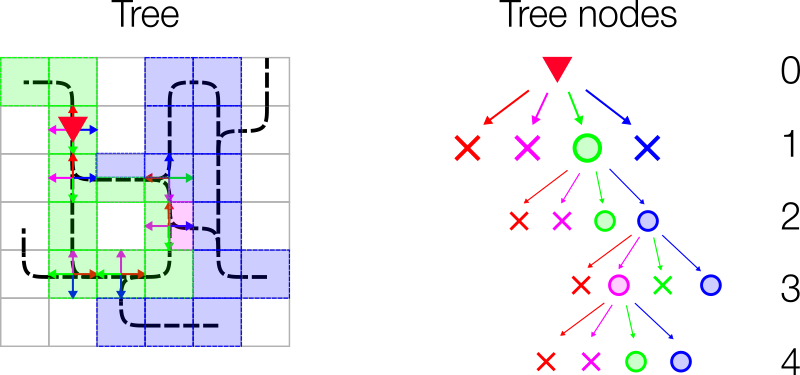
\includegraphics[width=\textwidth]{Images/tree.png}}
		\caption{The Flatland Tree Observation}
	\label{fig:tree}
\end{figure}



\subsubsection{Density Observation}

The custom Density Observation exploits Flatland's Shortest Path Predictor to assign each cell a value encoding information about if and when it will be occupied by a train. The values of all agents for a single cell are combined into a density value, depending on the time differences between the moments when the various agents occupy a given cell.

More specifically, each agent uses two matrices to learn: one matrix encodes the density map for the agent itself, while the other one is assigned density values depending on the other agent's predicted paths. Then the two matrices are stacked into a $w\times h\times 2$ matrix, where $w$ and $h$ are respectively the width and the height of the environment, which is then fed to a Convolutional Neural Network (CNN).%, as shown in Fig. \ref{fig:cnn}.%
The two matrices are stacked and not simply concatenated in order to preserve the spatial correspondency between the two matrices' density values. After 3 filtering layers of increasing size, the CNN output is flattened and passed to a standard Dueling DQN.

%\begin{figure}[h]
%	\centering
%		\fbox{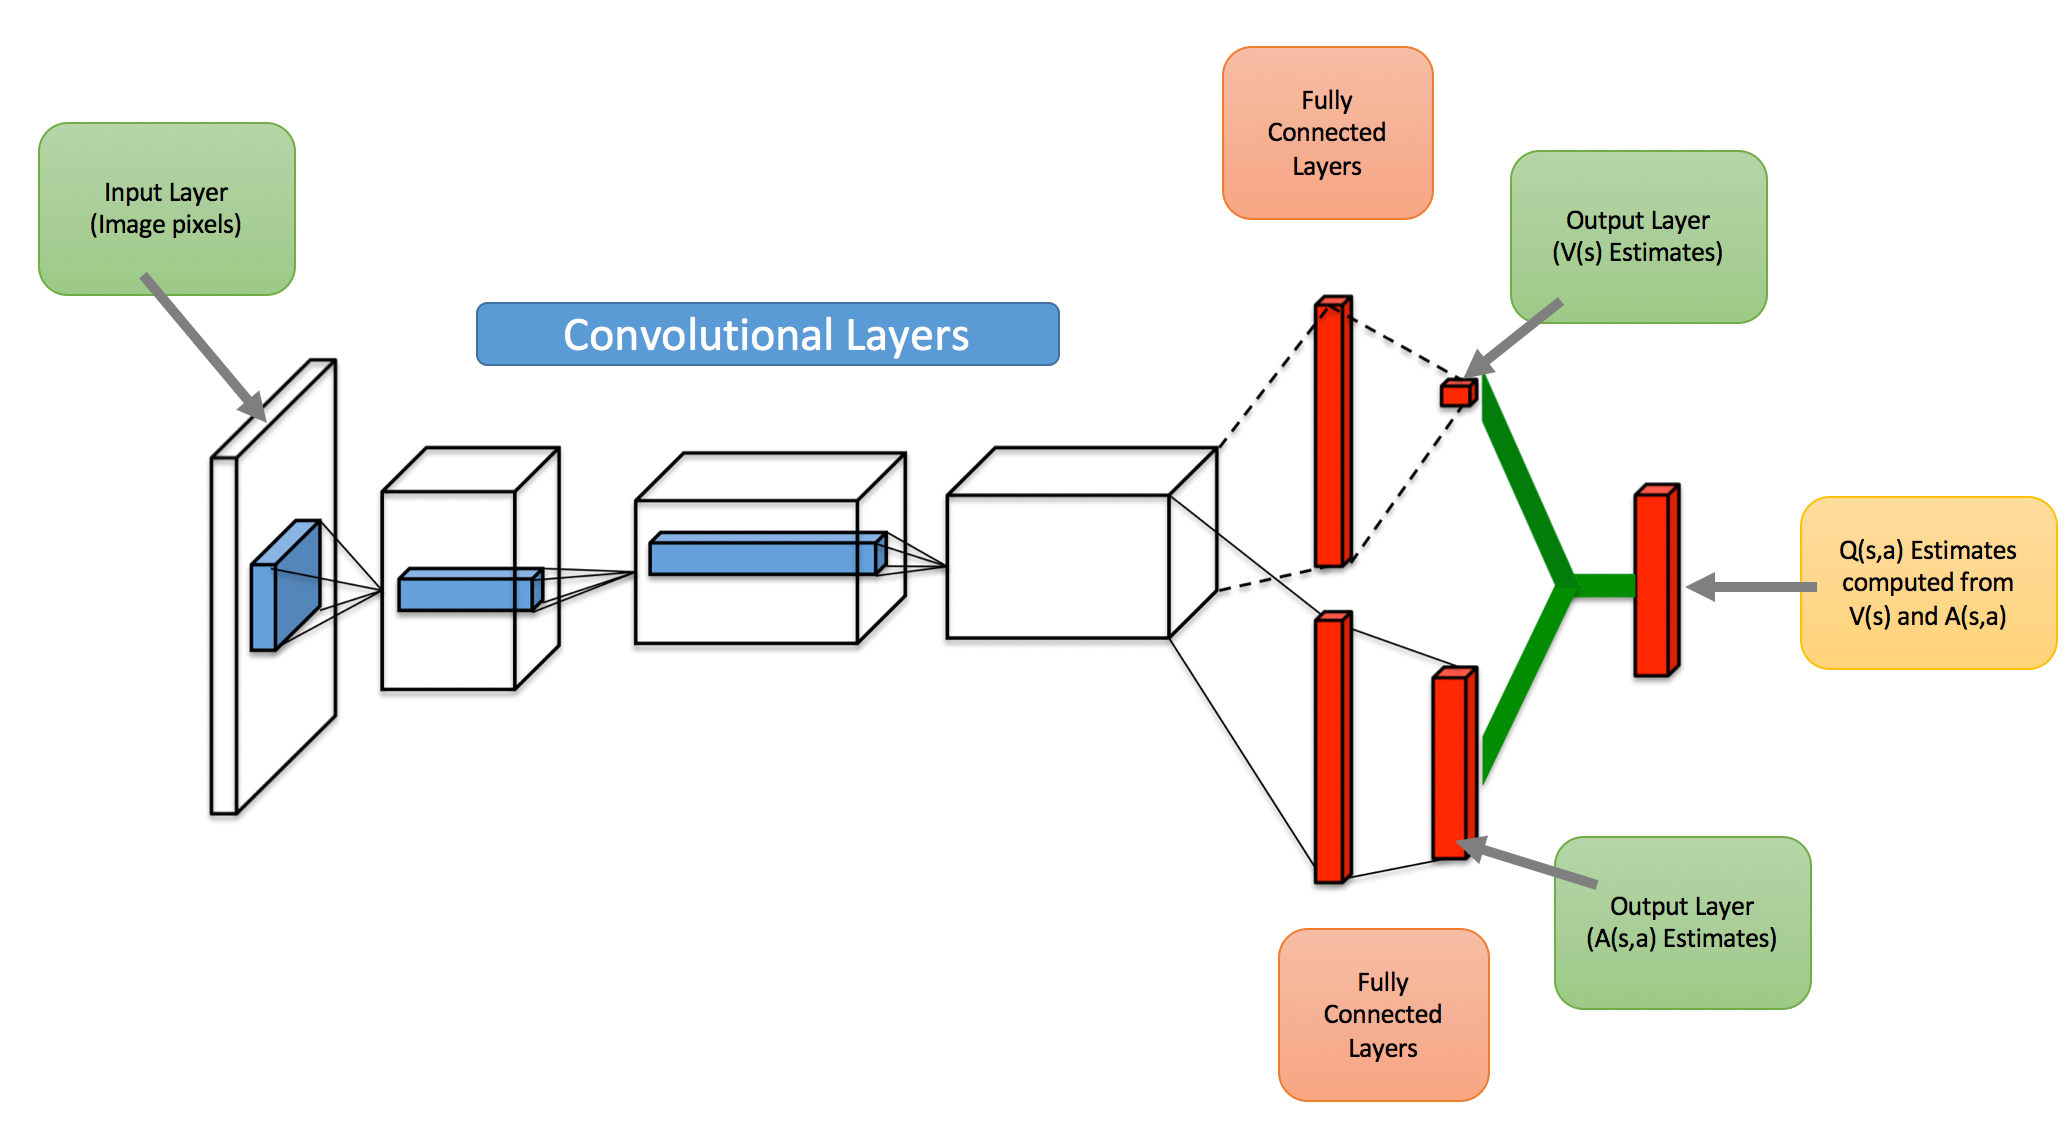
\includegraphics[width=\textwidth]{Images/cnn.png}}
%		\caption{CNN Dueling DQN used for the Density Observation}
%	\label{fig:cnn}
%\end{figure}

\subsection[Proximal Policy Optimization]{Proximal Policy Optimization \cite{ppo-algorithm, understanding-ppo}}

Proximal Policy Optimization (PPO) is a policy gradient-based method of reinforcement learning, designed to make some improvements on the Trust Region Policy Optimization (TRPO) algorithm, which in turn was designed to improve the Advantage Actor Critic (A2C) method. From the TRPO, the PPO inherits the importance sampling version of the policy loss function, which enables better sample efficiency, and which is expressed as follows:
\begin{equation}
	L^\mathrm{CPI}\left(\theta\right)=\mathbb{E}_t\left[\frac{\pi_\theta\left(a_t|s_t\right)}{{\pi_\theta}_\mathrm{old}}A_t\right]=\mathbb{E}_t\left[r_t\left(\theta\right)A_t\right],
\end{equation}
where the superscript $\mathrm{CPI}$ stands for ``Conservative Policy Iteration''. This loss function is an improvement of the one expressed by the A2C method. The policy loss indeed is no more subjected to the so-called ``destructively large policy updates'', typical of gradient-based methods, which maybe leads to update the parameters so far outside of the range, but now the policy gradient steps are limited, defining a ratio $r\left(\theta\right)$ between the action under the current policy and the action under the previous policy. PPO goes even further, introducing its main feature called ``clipped surrogate objective'', which can be expressed as follows:
\begin{equation}
	L^\mathrm{CLIP}\left(\theta\right)=\mathbb{E}_t\left[\min\left(r_t\left(\theta\right)A_t,\mathrm{clip}\left(r_t\left(\theta\right),1-\varepsilon,1+\varepsilon\right)A_t\right)\right].
\end{equation}

The loss function is given by the expectation computed over a minimum of two terms: a normal objective and a clipped objective. The key component comes from the second term where a normal objective is truncated with a clipping operation between $1-\varepsilon$ and $1+\varepsilon$, where $\varepsilon$ is a hyperparameter. Because of the $\min$ operator, the clipped objective behaves differently when the advantage estimate is positive or negative.

\begin{figure}[h]
	\centering
		\fbox{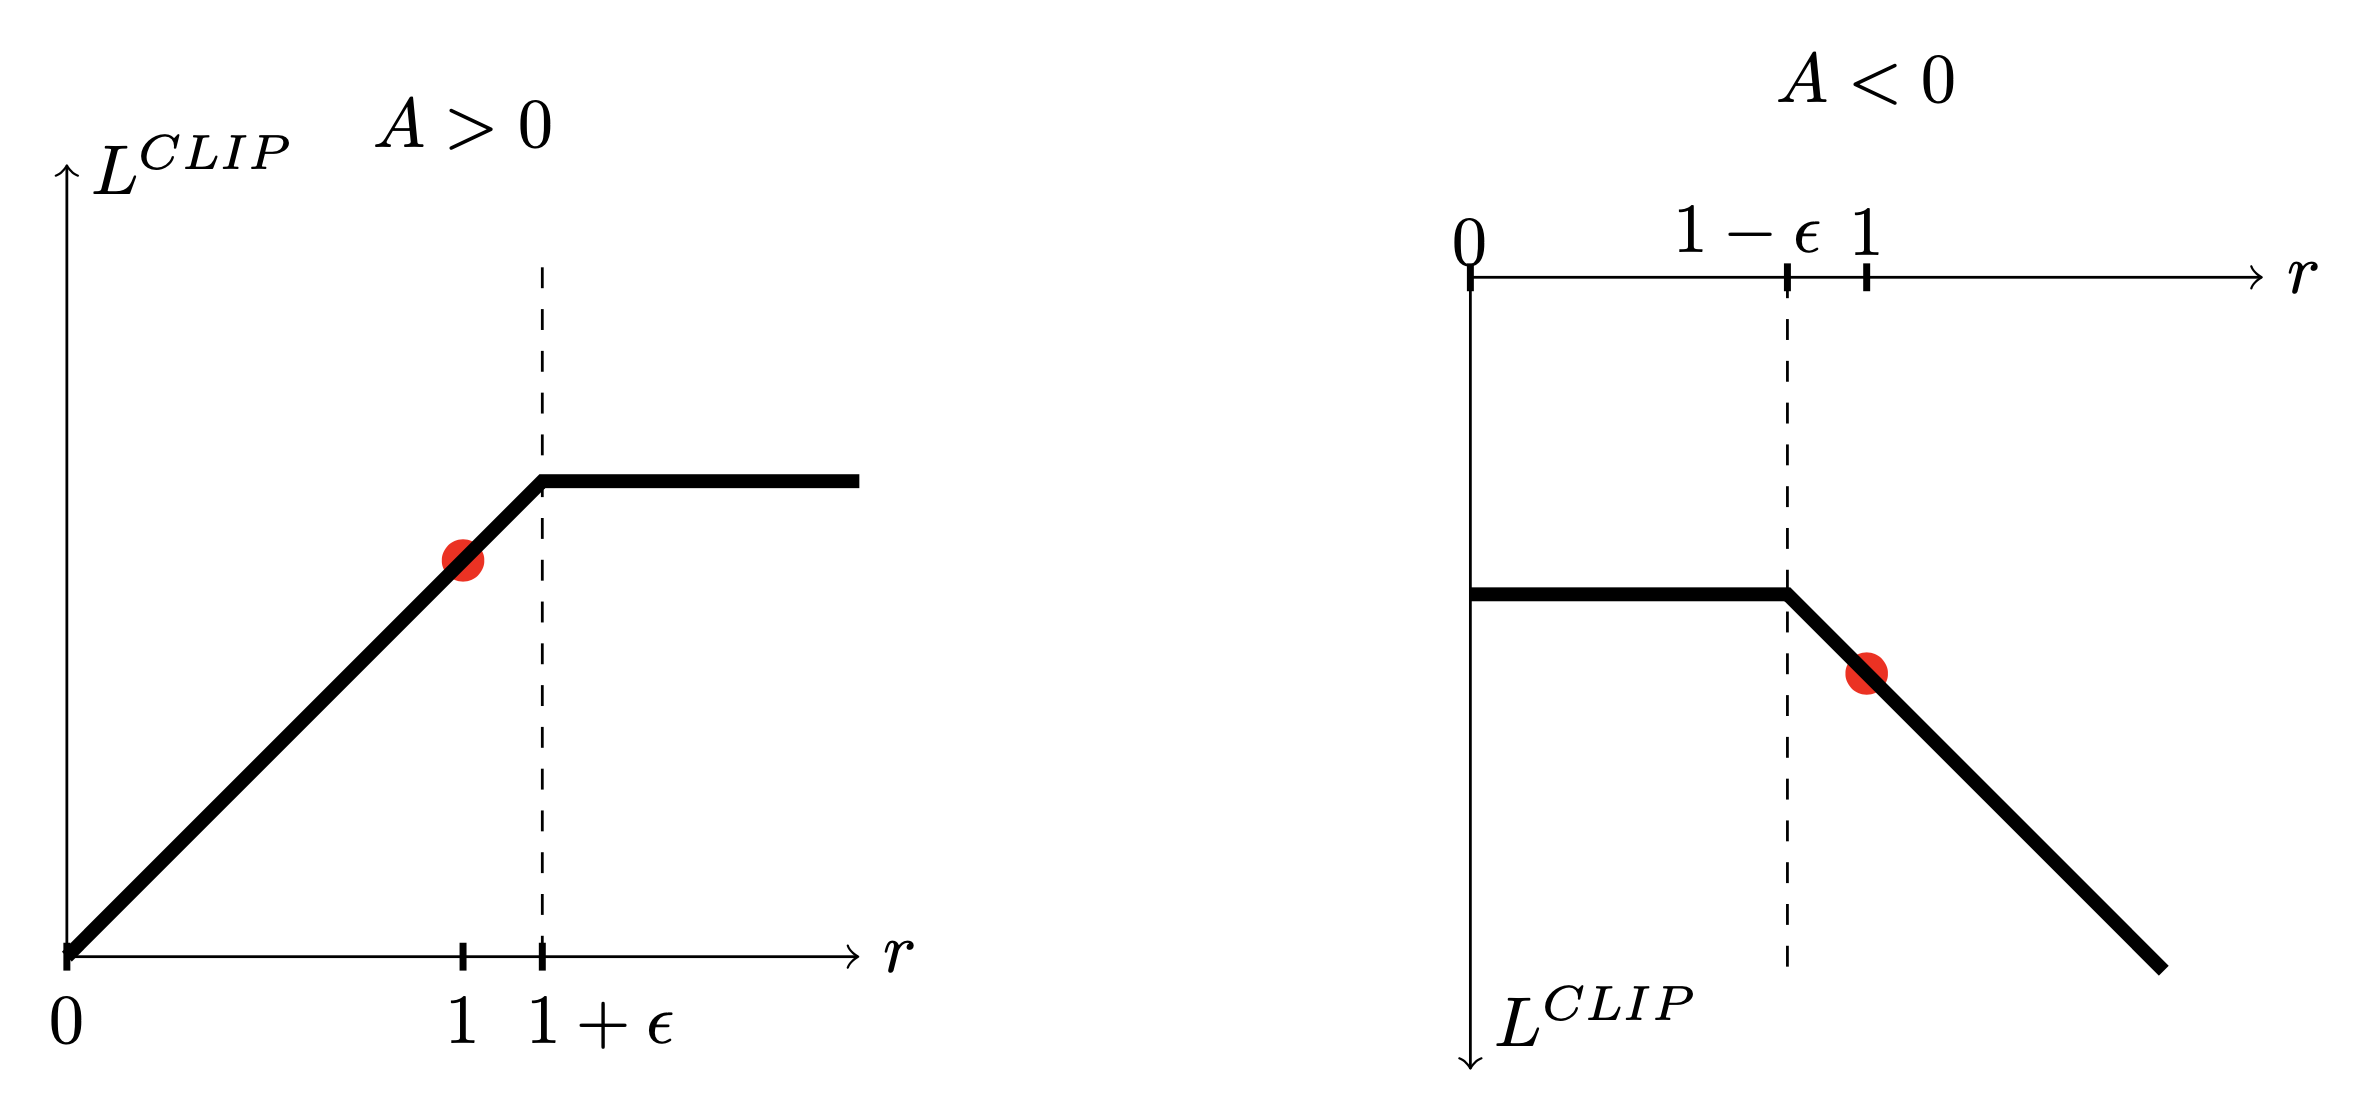
\includegraphics[width=\textwidth]{Images/clipped.png}}
		\caption[The $L^\mathrm{CLIP}$ function for positive and negative advantages]{The $L^\mathrm{CLIP}$ function for positive advantages $A>0$ and negative advantages $A<0$; the red circles show the starting points for the optimization}
	\label{fig:clipped}
\end{figure}

The effect of clipping is shown in Fig. \ref{fig:clipped}. On the left situation, when the selected action has a better-than-expected effect, the loss function flattens out when the action is much more likely under the current policy compare to the old one. This is done to prevent overdoing an action update by taking a step too far. The same happens to the graph on the right: the loss function flattens out when the action is much less likely under the current policy. This constraint is very powerful and avoid the computation of the additional KL constraint used in the TRPO in order to define a trust region, known to add overhead to optimization processes which sometimes leads to an undesirable training behavior. The total loss function for PPO then can be expressed as follows:
\begin{equation}
	L_t^{\mathrm{CLIP}+\mathrm{VF}+\mathrm{S}}\left(\theta\right)=\mathbb{E}_t\left[L_t^\mathrm{CLIP}\left(\theta\right)-c_1L_t^\mathrm{VF}\left(\theta\right)+c_2S\left[\pi_\theta\right]\left(s_t\right)\right],
\end{equation}
where $c_1$ and $c_2$ are hyperparameters that weigh the various components of the loss, $S$ denotes an entropy bonus (added to push the policy to behave more spontaneously until the other part of the objective starts dominating and so encouraging greater exploration), and $L_t^\mathrm{VF}$ is a squared-error loss (with the latter two terms identical to the components in A2C and with signs introduced to convert a maximization function to a minimization function).




\clearpage
\section{Results}

All training runs are performed with the following environment:
\begin{itemize}
	\item 3 agents;
	\item Width $w = 30$;
	\item Height $h = 30$;
	\item 2 cities;
	\item Maximum 2 rails between cities;
	\item Maximum 2 rails inside each city.
\end{itemize}

Experiment tracking is performed using the Weights and Biases tool \cite{wandb}.

All graphs show the number of steps on the $x$ axis and the average completion on the last 100 runs. The plots are smoothed with Weights and Biases's Gaussian filter with a power of $50$.




\clearpage

\subsection{Deep Q-Network agents}

The plot shown in Fig. \ref{fig:plot-dqn} represents 3 runs with different DQN agents and the following fixed settings:
\begin{itemize}
	\item $\varepsilon$-Greedy action selector;
	\item Standard Experience Replay;
	\item Tree Observation.
\end{itemize}


\begin{figure}[H]
	\centering
		\fbox{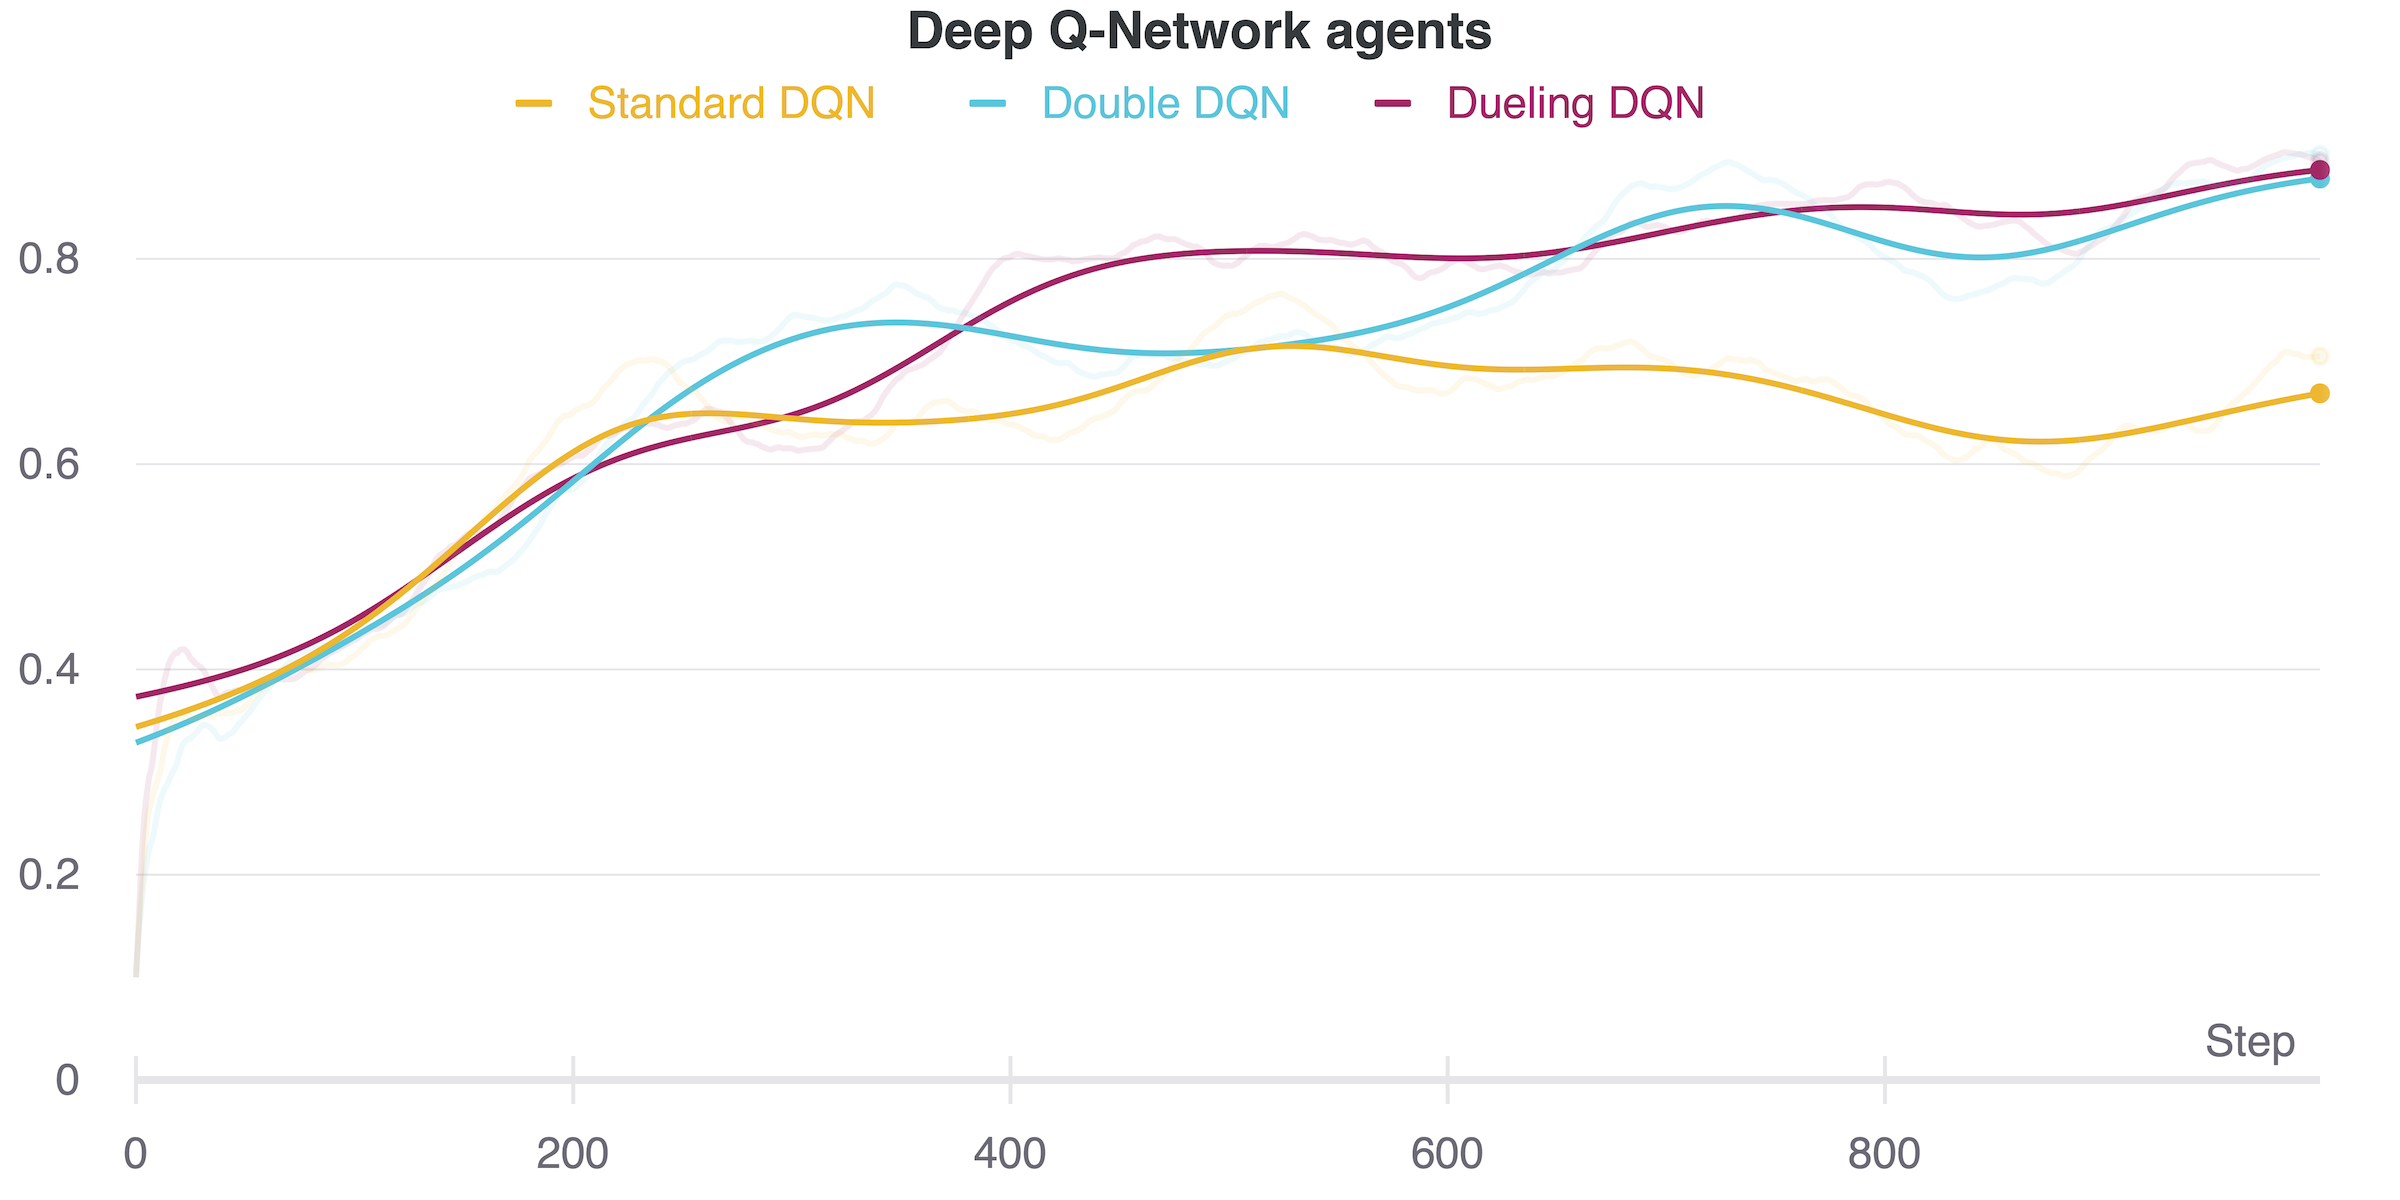
\includegraphics[width=\textwidth]{Images/plot-dqn.png}}
		\caption{Deep Q-Network agents}
	\label{fig:plot-dqn}
\end{figure}

The Standard DQN performs much worse compared to the Double and Dueling DQN agents. This is in line with what is expected according to the theory exposed in Section \ref{sec:dqns}.


\clearpage

\subsection{Action selectors}

The plot shown in Fig. \ref{fig:plot-action-selectors} represents 3 runs with different action selectors and the following fixed settings:
\begin{itemize}
	\item Standard DQN agent;
	\item Standard Experience Replay;
	\item Tree Observation.
\end{itemize}


\begin{figure}[H]
	\centering
		\fbox{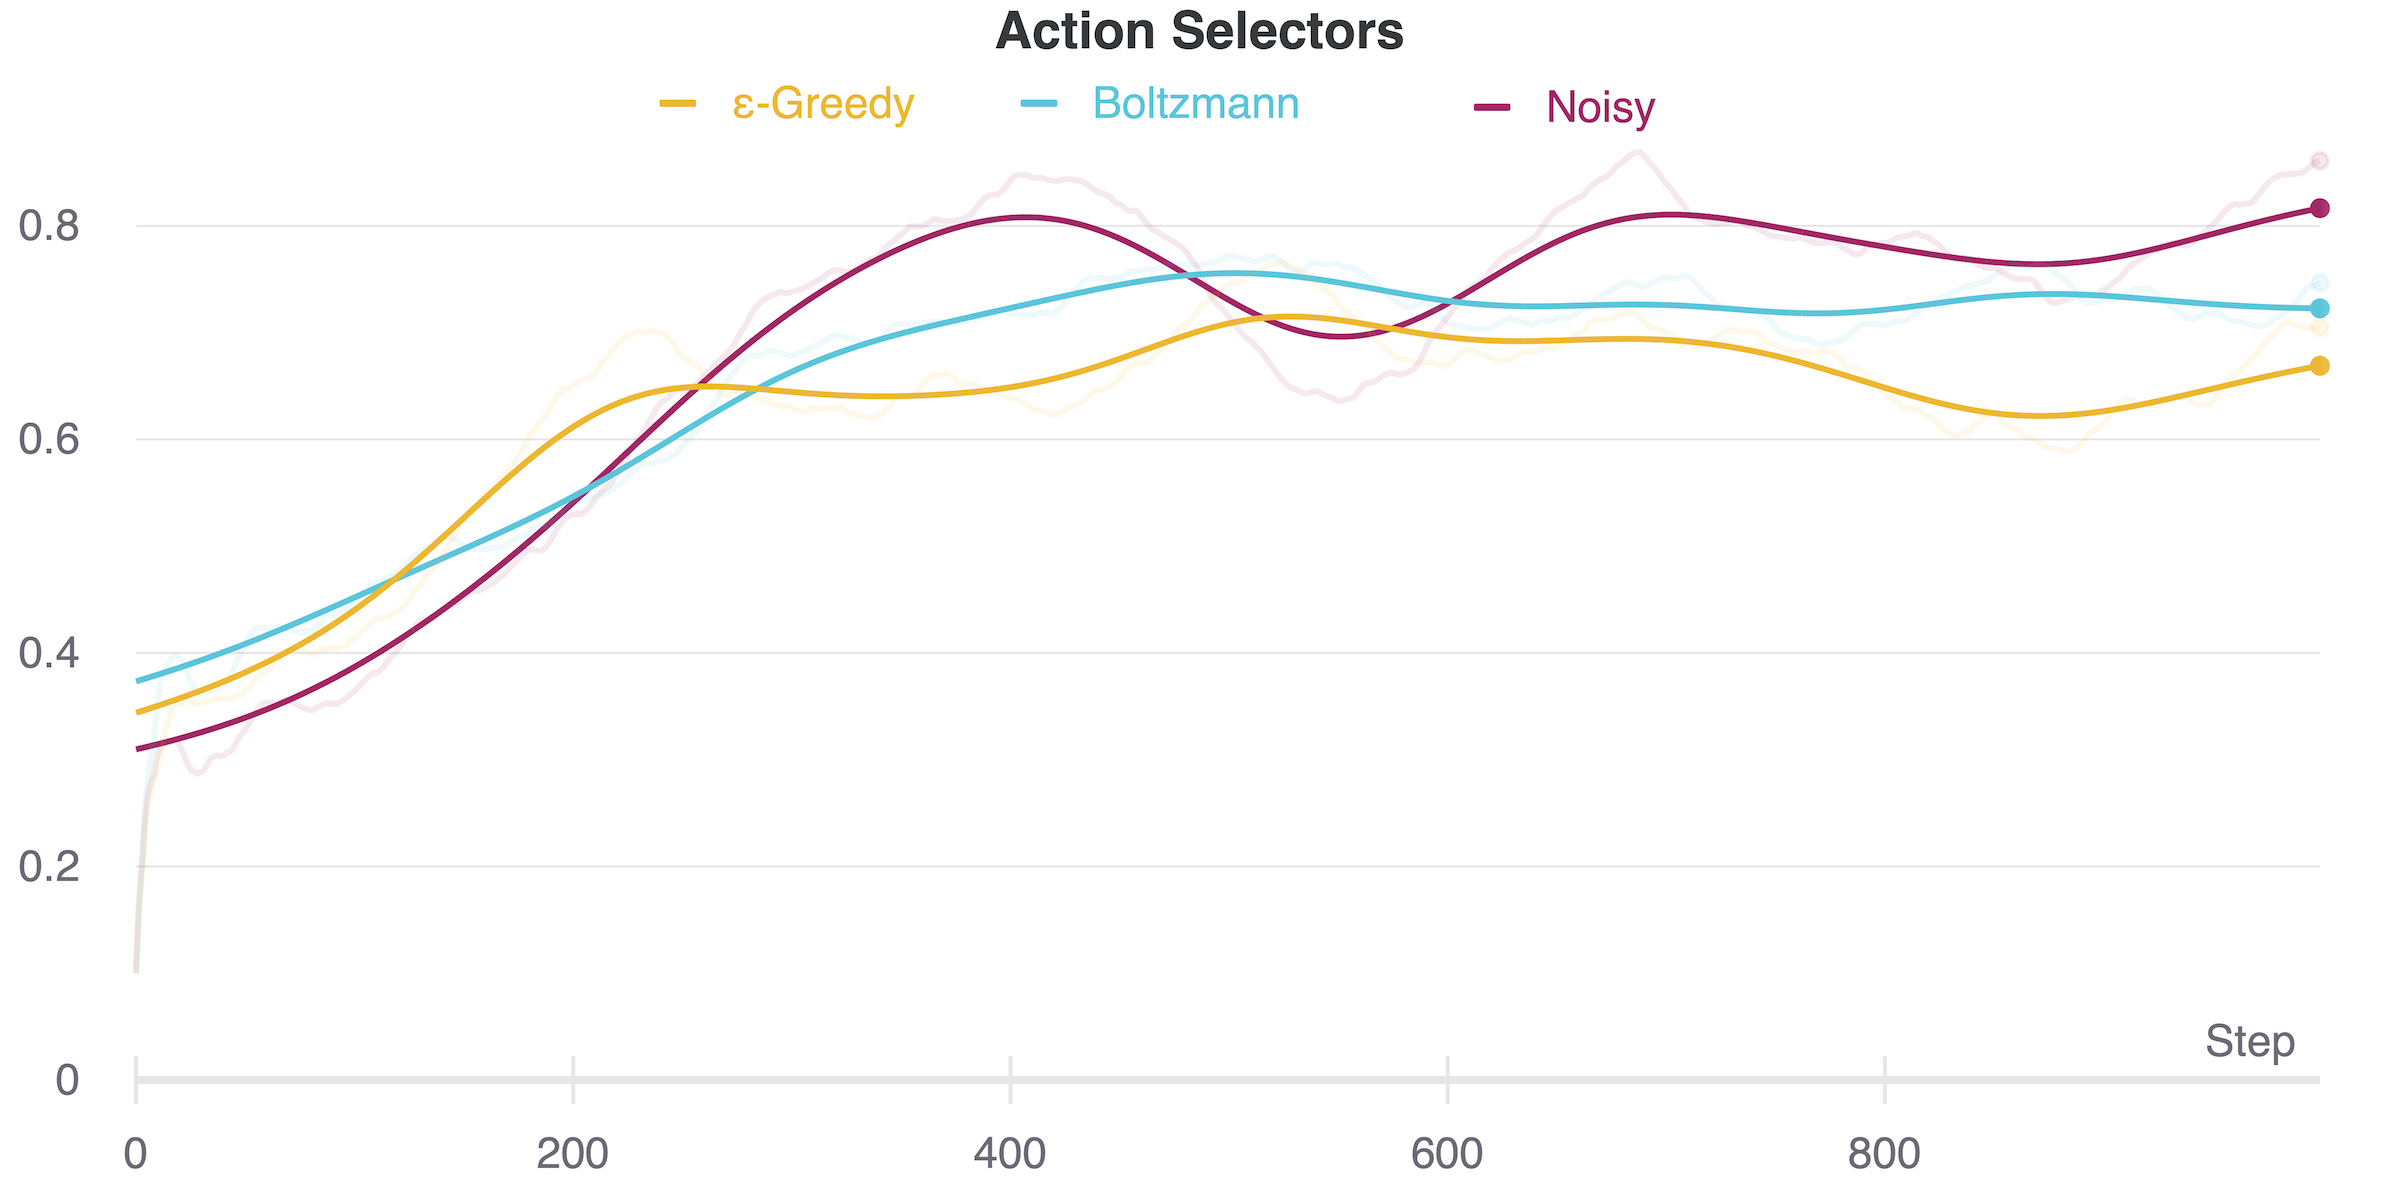
\includegraphics[width=\textwidth]{Images/plot-action-selectors.png}}
		\caption{Action selectors}
	\label{fig:plot-action-selectors}
\end{figure}

The Noisy action selector is clearly the best of the 3, with $\varepsilon$-Greedy and Boltzmann being quite close to each other. Again, these results are consistent with the expectations, given the content of Section \ref{sec:action-selectors}.

\clearpage
\subsection{Experience Replay}

The plot shown in Fig. \ref{fig:plot-experience-replay} represents 2 runs with different Experience Replay paradigms and the following fixed settings:
\begin{itemize}
	\item Standard DQN agent;
	\item $\varepsilon$-Greedy action selector;
	\item Tree Observation.
\end{itemize}

\begin{figure}[H]
	\centering
		\fbox{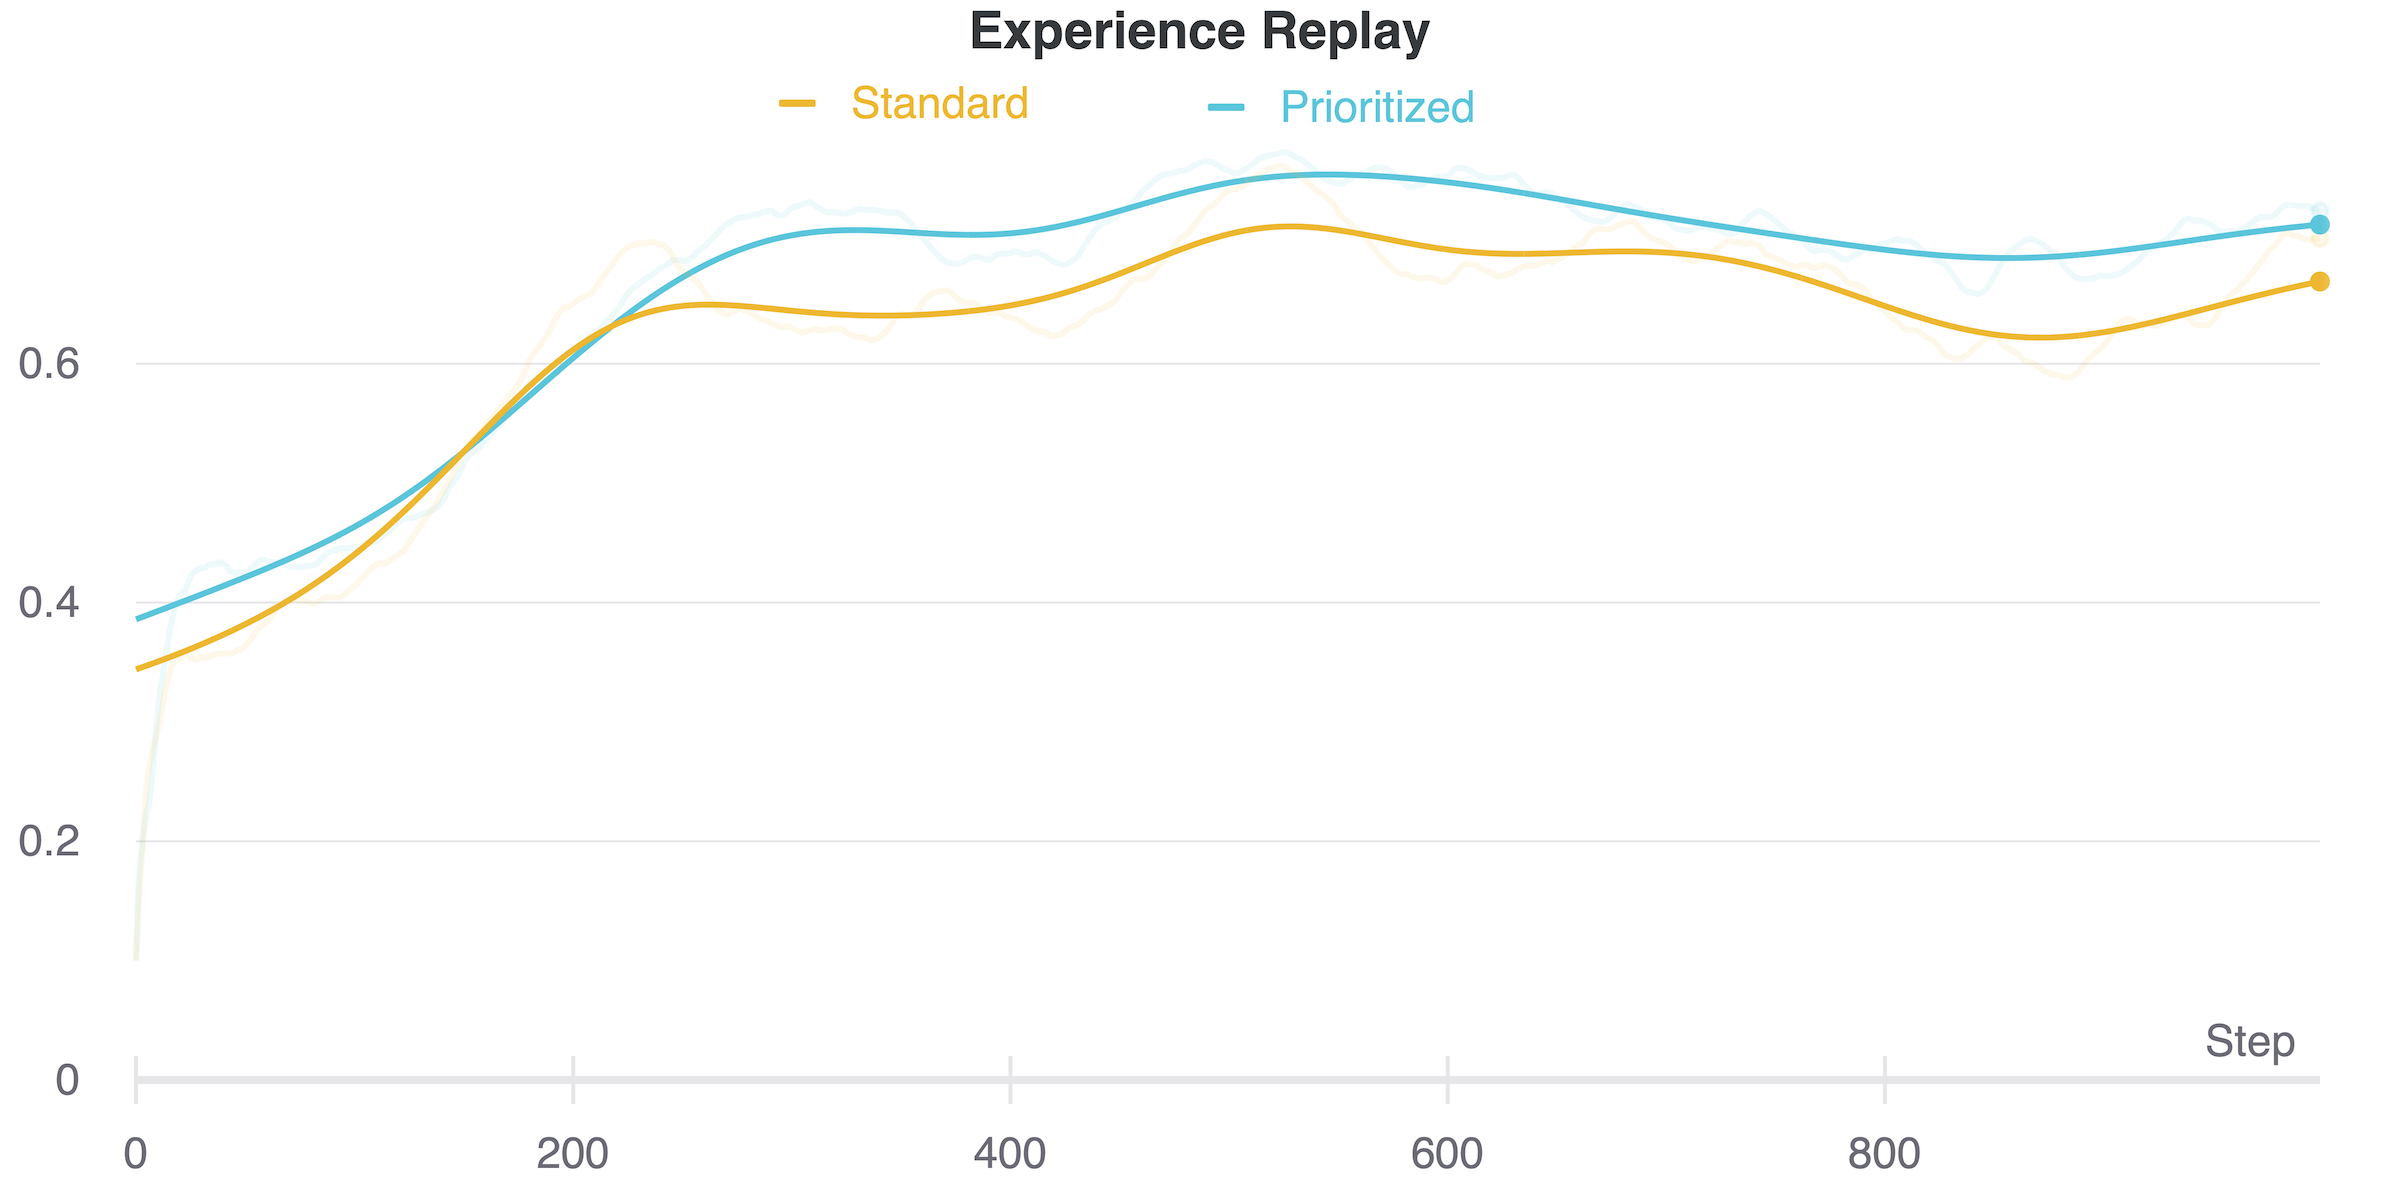
\includegraphics[width=\textwidth]{Images/plot-experience-replay.png}}
		\caption{Experience Replay}
	\label{fig:plot-experience-replay}
\end{figure}

The Prioritized Experience Replay run performs slightly better than the Standard one, in line with the theory of Section \ref{sec:experience-replay}.

\clearpage
\subsection{Observations}

The plot shown in Fig. \ref{fig:plot-observations} represents 2 runs with different observations and the following fixed settings:
\begin{itemize}
	\item Dueling DQN agent;
	\item $\varepsilon$-Greedy action selector;
	\item Standard Experience Replay.
\end{itemize}

\begin{figure}[H]
	\centering
		\fbox{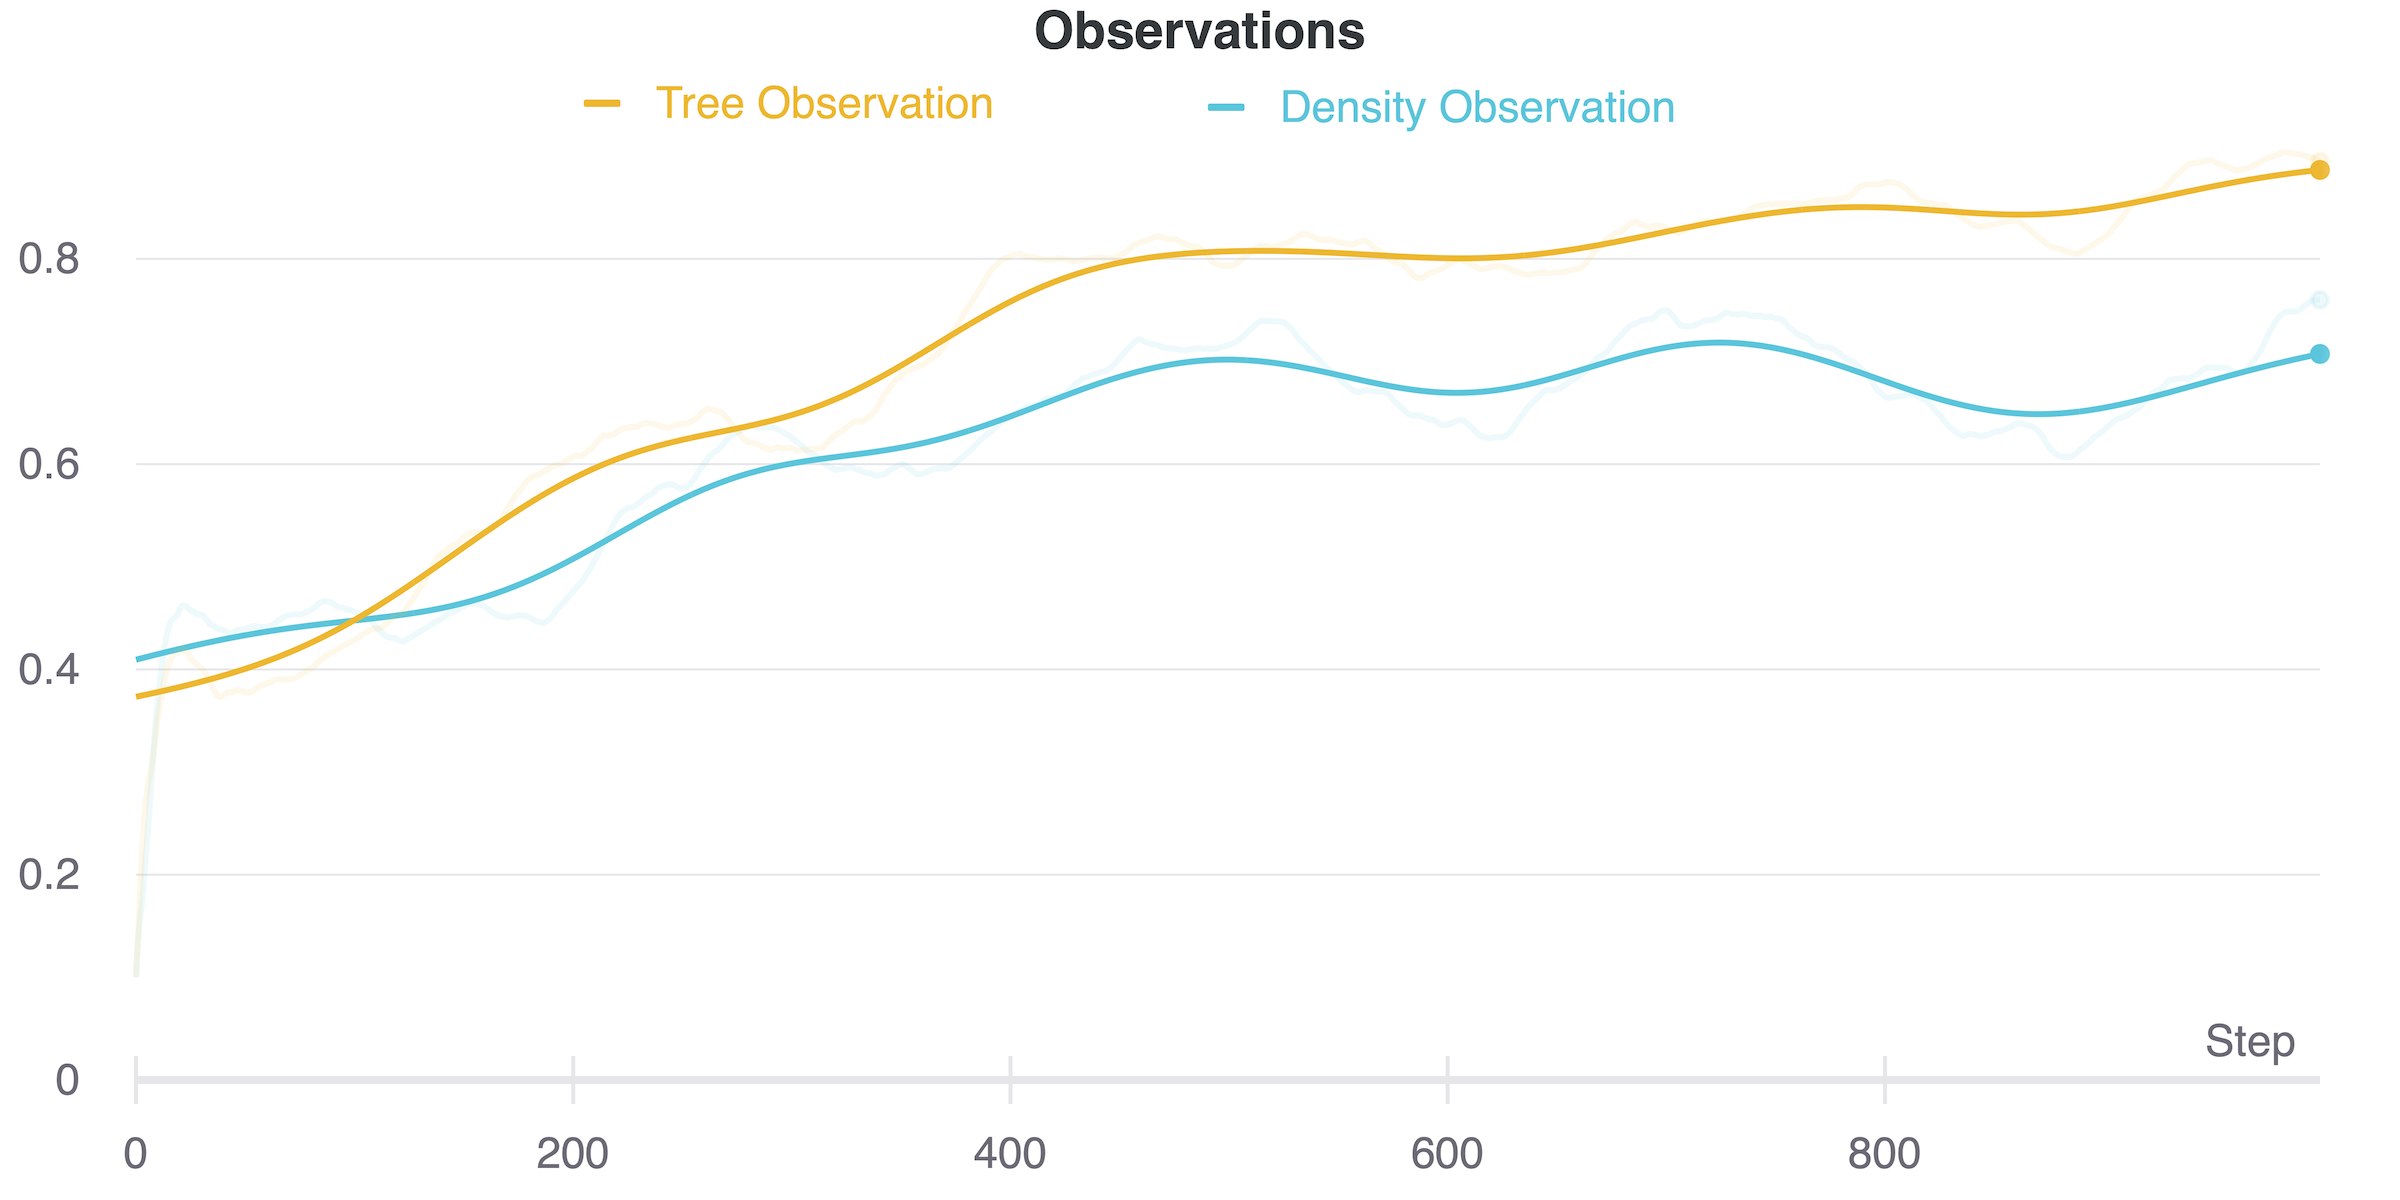
\includegraphics[width=\textwidth]{Images/plot-observations.png}}
		\caption{Observations}
	\label{fig:plot-observations}
\end{figure}

Even though it is a custom observation, Density Observation did not perform as bad as expected, despite being clearly worse than the Tree Observation run, which is also the reason why Tree Observation was preferred for all the other runs.

\clearpage
\subsection{Proximal Policy Optimization}

The plot shown in Fig. \ref{fig:plot-ppo} represents 3 runs with different PPO parameters. The legend labels correspond to a triple of $\varepsilon/c_1/c_2$.


\begin{figure}[H]
	\centering
		\fbox{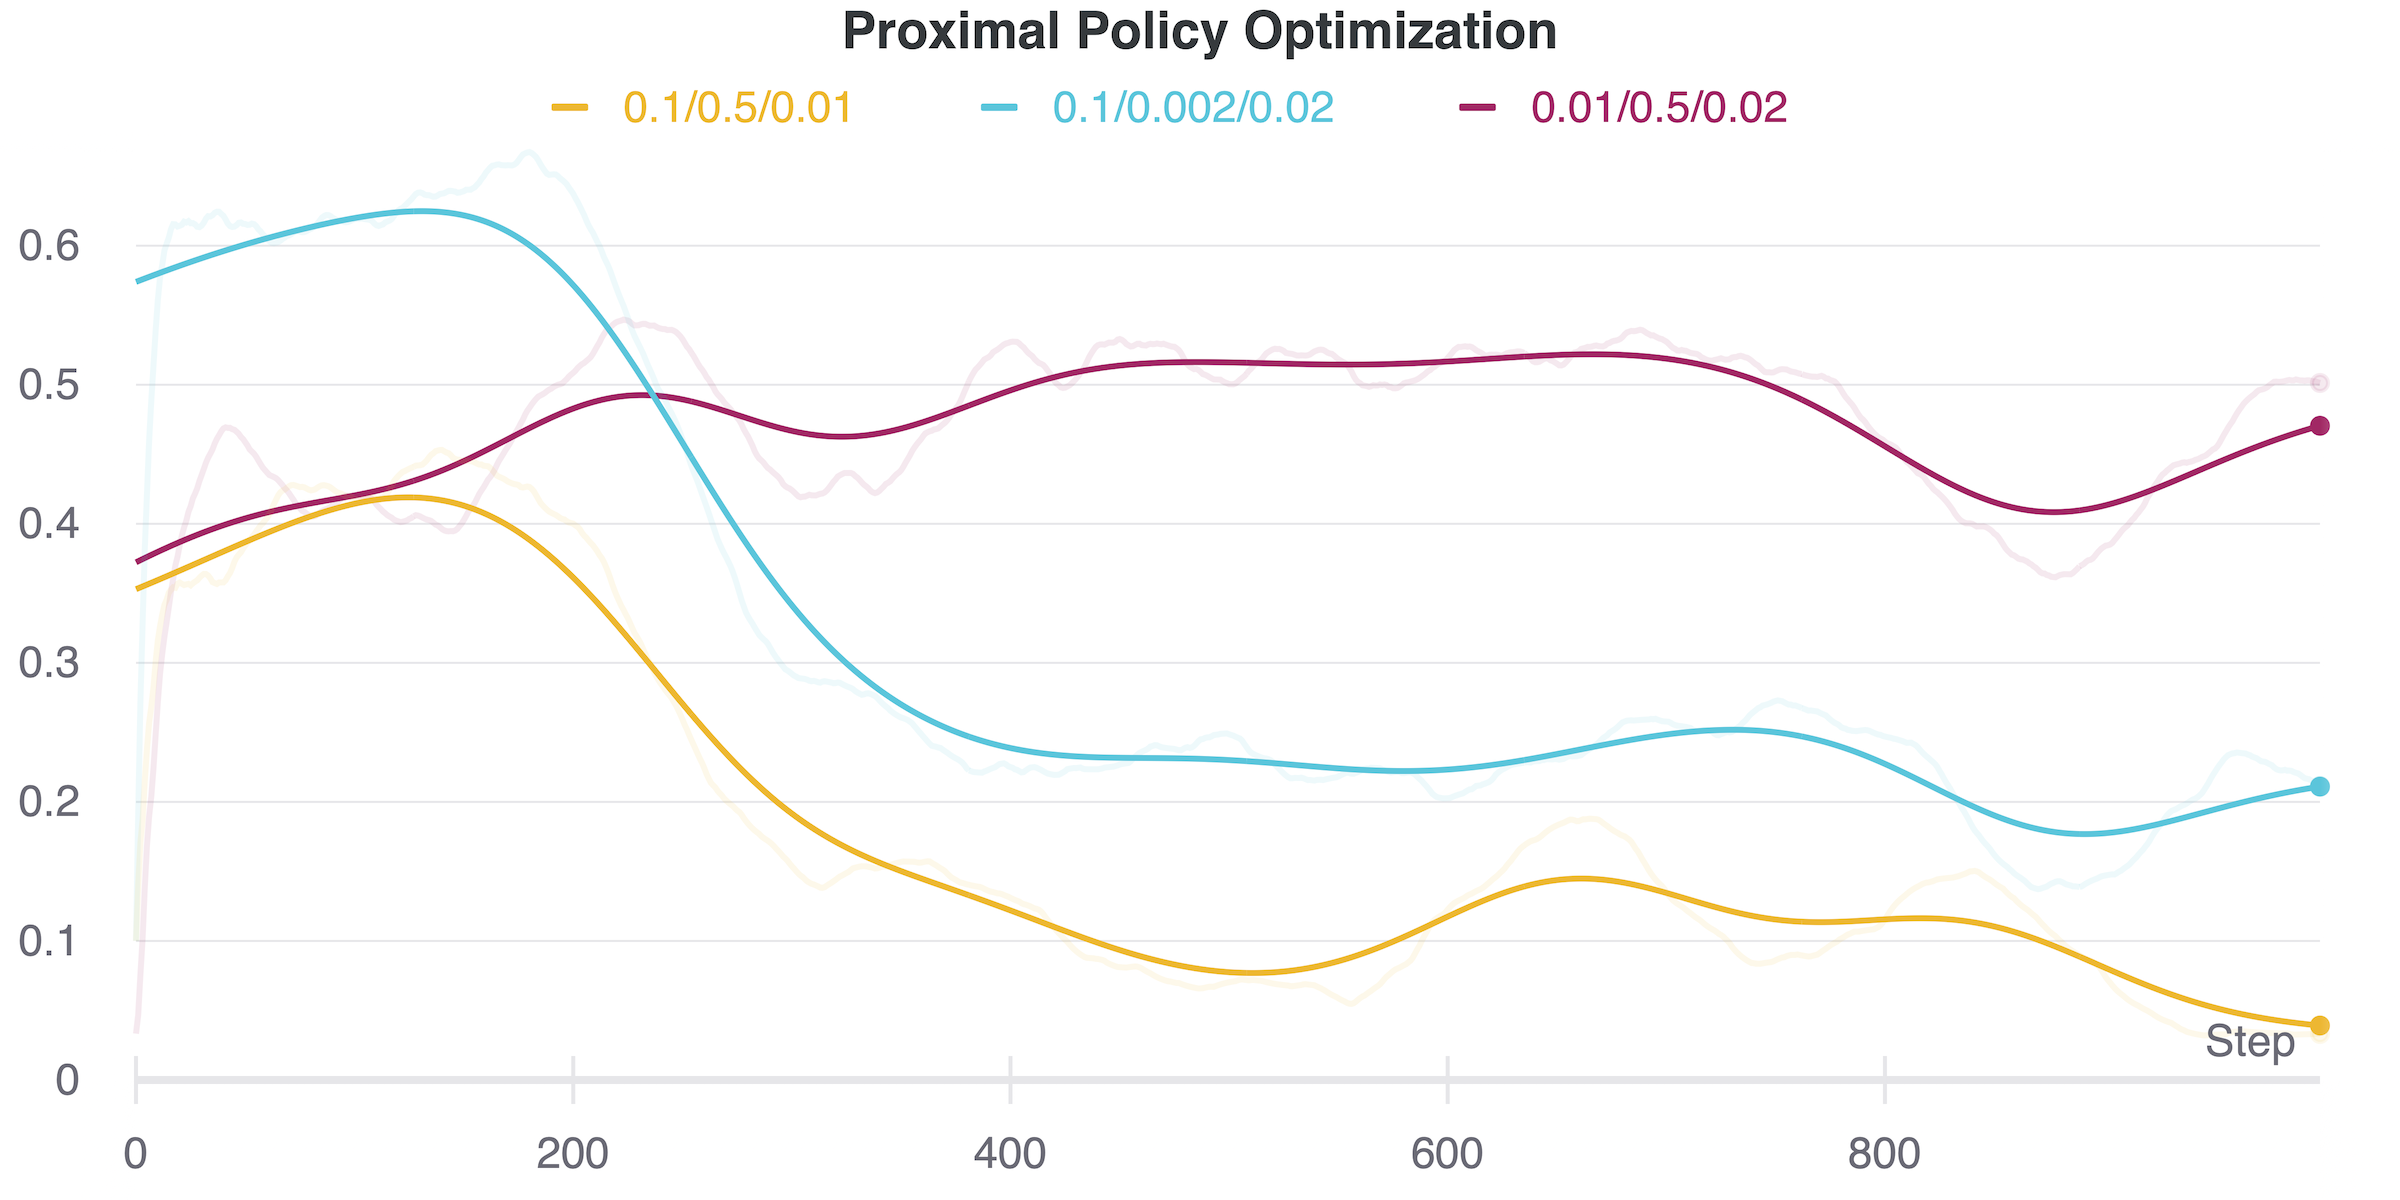
\includegraphics[width=\textwidth]{Images/plot-ppo.png}}
		\caption{Proximal Policy Optimization}
	\label{fig:plot-ppo}
\end{figure}

Using a bigger $\varepsilon$ value ($0.1$), when the agent starts to go down a bad path it is unable to recover, resulting in a swift decrease of completion percentage. This behavior is particularly evident when using a small entropy weight ($c_2$). On the contrary, using a small $\varepsilon$ value ($0.01$) and a big entropy weight ($0.02$) helps recovering after a bad path is taken, giving the best results. In any case, the performance of PPO methods is clearly worse than the runs shown in previous plots.






















\clearpage
\printbibliography[heading=bibintoc]

\end{document}